\chapter{Performance Evaluation}
%Here should be an introduction of what we will test (the emulator and/or the protocol). 

To evaluate the designed system a few key parameters are set as main pointers. This include the amount of users and the configurability of the solution, as well as it physical limitations. The system is then used to test the NB-IoT protocol, to show the usability of the solution. Some of these evaluation points have been described prior but a complete list is provided in the following section.

\section{Evaluation Points}
%Here should be a list of all requirement that is tested and criteria for passed not passed. 
The key parameters can be spilt into two groups: the emulator and the protocol. These groups are independent of each other in the sense that any other emulator should reveal the same results for the same protocol, given the same parameters.

\begin{itemize}
\item Emulator
	\begin{enumerate}
	\item Amount of users %(CPU,RAM) 
		\begin{itemize}
		\item Support TBD active users and TBD users total
		\end{itemize}
	\item Configurability  %(Channel, Number of UEs, etc.)
		\begin{itemize}
		\item Changeable parameters: Channel type, path loss, number of devices, data profile
		\end{itemize}
	\item Limits 
		\begin{itemize}
		\item Should support a output power up to 23 dB with a range of TBD dB
		\item Should support the frequency range from TBD to TBD and a bandwith up to TBD
		\end{itemize}
	\end{enumerate}
\item Protocol
	\begin{enumerate}[resume]
	\item  Ultra-low Complexity Devices
		\begin{itemize}
		\item The \gls{UE} has a sample rate of 240 KHz
		\item Only supports \gls{TBCC}
		\item Half-duplex
		\item Uses \gls{SISO} connection
		\end{itemize}
	\item Improved Coverage
		\begin{itemize}
		\item Support a \gls{MCL} of 164 dB
		\item Improve coverage by introducing \gls{CE} levels 
		\end{itemize}
	\item Support Massive Number of Devices 
		\begin{itemize}
		\item Support 52547 devices per cell-site sector based on a TBD data profile
		\end{itemize}
	\item Improved Power Efficiency
		\begin{itemize}
		\item  Achieve a battery life time of 10 years with a battery capacity of 5 Wh
		\item Using \gls{CE} to minimize Power amplifier backoff increasing efficiency
		\item Utilize \gls{cDRX}, \gls{eDRX} and \gls{PSM} to increase efficiency
	\end{itemize}
	\item Deployment flexibility
		\begin{itemize}
		\item The system should be able to be deployed inside legacy \gls{LTE}.
		\item The system should be able to be deployed as a stand alone solution.
		\end{itemize}
	\end{enumerate}
\end{itemize}
%\item Massiveness
%	\begin{enumerate}
%	\item Time to connect vs. connection request per second 
%	\item Data rate vs. number of users
%	\item Spectrum use vs. number of users
%	\item Interference level vs. number of users
%	\end{enumerate}
%\item Power
%	\begin{enumerate}
%	\item Energy consumption for attach.
%	\item Energy consumption vs. data rate
%	\item Energy consumption vs. coverage level
%	\item Energy consumption vs. operation mode
%	\item Energy consumption vs. number of UEs
%	\item Energy consumption vs. UE state (Connected (cDRX), eDRX, PSM, Off)
%	\end{enumerate}
%\end{enumerate}


Based on both the focus explained in \autoref{ch:Introduction} as well as some issues with the emulator explained TBD. The only points that is actually tested are: \todo{check if this is correct later}

\begin{itemize}
\item Emulator
	\begin{enumerate}
	\item[1.] Amount of users %(CPU,RAM) 
	\item[2.] Configurability %(Channel, Number of UEs, etc.)
%	\item[3.] Power control 
	\end{enumerate}
\item Protocol
	\begin{enumerate}
%	\item[4.] Ultra-low Complexity Devices
%	\item[5.] Improved Coverage
	\item[6.] Support Massive Number of Devices 
	\item[7.] Improved Power Efficiency
	\item[8.] Deployment flexibility
	\end{enumerate}
\end{itemize}

\newpage

\section{General Test Setup}
%Here should be a description of the general setup (including figure) used in all test and a list of baseline values for all parameters. Including physical setup, BSE, UEE.

The general way to setup the emulator is described here, some deviations occurs depending on the actual use of the system. A full setup is only needed when an external device is tested under the influence of a large number of interfering devices. The full setup can be seen in \autoref{fig:General_test_setup}.

\begin{figure}[H]
\centering
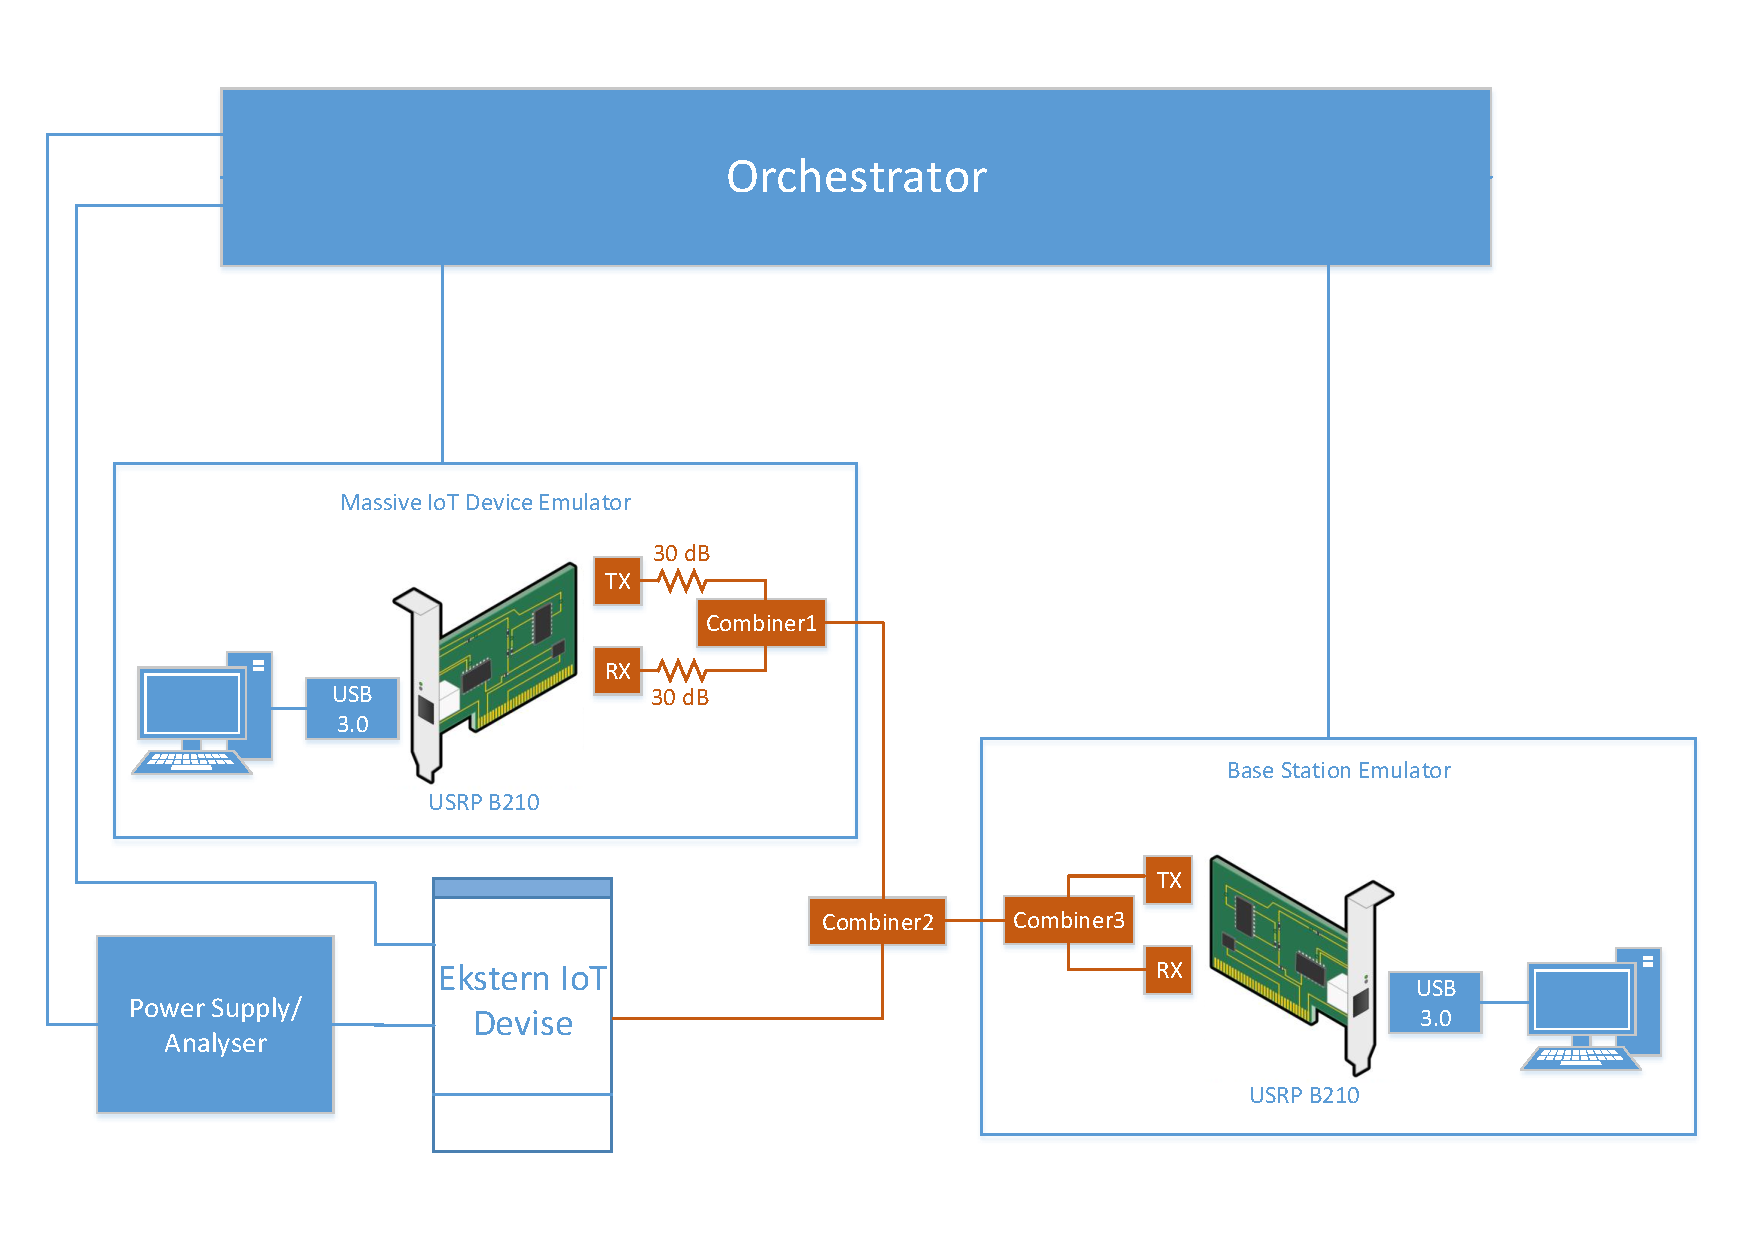
\includegraphics[width=\textwidth]{figures/General_test_setup.pdf}
\caption{General test setup, blue lines are control connections, orange lines are RF connections.}
\label{fig:General_test_setup}
\end{figure}

As seen in \autoref{fig:General_test_setup}, a \gls{TAP} orchestrator maintain the system. The orchestrator has a \gls{LAN} connection with each of the other elements with the exception of the external IoT device which is dependent on the device but typically is a serial connection. The \gls{PSU}s connection with the external IoT device is plain wires used to power on and analyse the power consumption of the device. Both the massive IoT device emulator as well as the external IoT device is connected to a combiner using RF SMA cables, this combiner is connected to the \gls{BSE} also using a RF SMA cable. 

The massive IoT device emulator PC is connected using USB 3.0 to the USRP B210. Mounted on the TX1 and RX1 port is a 30 dB attenuator which is connected to a combiner using RF SMA cables the output of the combiner acts as the output of the emulator.

The \gls{BSE} is interchangeable if the UXM is used TxRx1/Rx1 on RF Transceiver A is used as input. If the Amarisoft BSE is used the input is a combiner connected to the TX1 and RX1 ports on a USRP B210 using RF SMA cables, which is connected to the PC using a USB 3.0 connector.

The initial settings of each component in the system can be seen in \autoref{tab:setup_parameters}.

\begin{table}[H]
\captionsetup{belowskip=0em}
\noindent
\centering
%\resizebox{!}{0.5\textheight}{
\begin{minipage}[t]{0.48\textwidth}
\begin{tabular}{|p{4cm}|p{2cm}|}
\hline
\multicolumn{2}{|c|}{\textbf{Power Supply/Analyser}}                         \\ \hline
Enable             & Off            \\ \hline
Volt               & 3.6 V          \\ \hline
Ampere             & 2.5 A          \\ \hline
Sample interval	   & 100 $\mu$s		\\ \hline
\multicolumn{2}{c}{}\\ \hline
\multicolumn{2}{|c|}{\textbf{Massive IoT Emulator}}                          \\ \hline
\textbf{Parameter} & \textbf{Value} \\ \hline
Number of devices  & 0              \\ \hline
Rx gain            & 40 dB          \\ \hline
Tx gain            & 40 dB          \\ \hline
R14                & False          \\ \hline
Dl\_EARFCN         & 6240           \\ \hline
UE\_category       & Nb1            \\ \hline
\end{tabular}
%\caption{Initial values of the parameters in the emulator.}
\end{minipage}% 
\hfill
\begin{minipage}[t]{0.48\textwidth}
\begin{tabular}{|p{4cm}|p{2cm}|}
\hline
\multicolumn{2}{|c|}{\textbf{Ekstern IoT device}}                            \\ \hline
Enable             & Off            \\ \hline
Dl\_EARFCN         & 6240           \\ \hline
\multicolumn{2}{c}{}\\ \hline
\multicolumn{2}{|c|}{\textbf{Base Station Emulator}}                         \\ \hline
Cell type          & NB-IoT         \\ \hline
Number of cells    & 1              \\ \hline
Operation mode     & Standalone     \\ \hline
Dl\_EARFCN         & 6240           \\ \hline
Cell ID            & 0              \\ \hline
Tx gain            & 89 dB          \\ \hline
R14                & False          \\ \hline
nprach\_detect\_ threshold  & 19 dB  \\ \hline
\end{tabular}
%\caption{Initial values of the parameters in the emulator.}
%\label{tab:setup_parameters}
\end{minipage}
\caption{Initial values of the parameters in the emulator.}
\label{tab:setup_parameters}
\end{table}


\section{Evaluation}
%Here should be a step by step procedure of all test for all requirements, maybe put tapplans in appendix.

%\subsection{Amount of Devices}

\subsection{Configurability}

%\subsection{Power Control}

%\subsection{Ultra-low Complexity Devices}

%\subsection{Improved Coverage}

%\subsection{Support Massive Number of Devices}

\subsection{Improved Power Efficiency}
\subsubsection{Test Overview}
From \appref{app:bat_model} it can be seen that to estimate the battery life time of a device the following parameters is needed.
\begin{itemize}
%\item $P_{device}$
%\item $E_{modem,on}$
\item $E_{sync}$
\item $E_{attach}$
\item $P_{tx}$
\item $P_{eDRX}$
\item $P_{PSM}$
\end{itemize}

With these informations the only thing needed is the data profile, the same models are used here as in \citep{Power_article}. Model 1 transmit every hour and Model 2 transmit every 24 hours, transmission size is 100 bytes for both models. %\todo{see if standards have some specified data profiles.}

From a measurement perspective some of these parameters can and should be measured together, these are $E_{sync}$ and $E_{attach}$. This is because these steps are depending on each other and can not be separated for the measurements only in the post processing. These are collectively referred to as $E_{conn}$ or energy to connect the device to the cell. 

To test these parameters the following setup is modified from \autoref{fig:General_test_setup} to the following:

\begin{figure}[H]
\centering
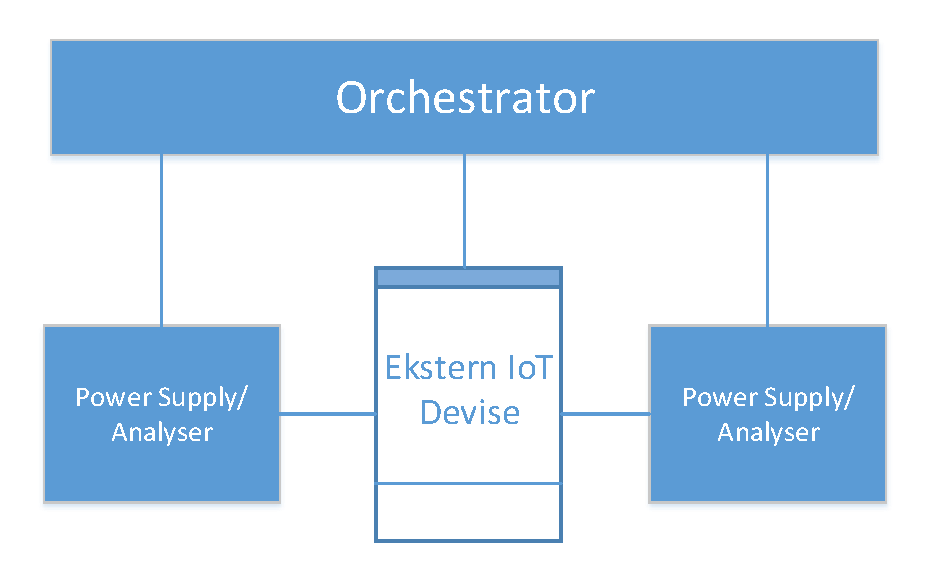
\includegraphics[width=0.5\textwidth]{figures/IPE_test_setup.pdf}
\caption{Setup used to test for the power efficiency of the \gls{DUT}'s}
\label{fig:IPE_test_setup}
\end{figure}

It should be noted that the \gls{DUT}'s in question have to power inputs, one for the device power and one for the RF modem power. Typically only the modem is connected to the power analyser. With the exception of measuring the device power where the the device power input is connected to the power analyser.

As the UXM is used as \gls{BSE} instead of Amarisoft the initial settings for this can be seen in \autoref{tab:UXM_initial_values}.

\begin{table}[H]
\centering
\begin{tabular}{|c|c|} \hline
\multicolumn{2}{|c|}{\textbf{UXM \gls{BSE}}} \\ \hline
Cell type			 & NB-IoT         \\ \hline
Number of cells		 & 1              \\ \hline
Operation mode		 & Standalone     \\ \hline
Host cell Dl\_EARFCN & 6240           \\ \hline
PRB offset			 & 0	          \\ \hline
Cell ID				 & 0              \\ \hline
Tx power			 & -80 dB/per 15 kHz \\ \hline
Repetition NPDSCH	 & 1	          \\ \hline
Max Repetition NPDCCH & 4	          \\ \hline
Repetition NPUSCH	 & 1	          \\ \hline
Repetition NPRACH	 & 1	          \\ \hline
CP format			 & Normal         \\ \hline
Pmax				 & 23 dBm         \\ \hline
\end{tabular}
\caption{Initial parameters of the UXM}
\label{tab:UXM_initial_values}
\end{table}

%\subsubsection{Device Power Consumption}
%
%To measure the device power, the power input to the device is used in the setup. The test is performed using the following procedure:
%
%\textbf{Test Procedure}
%\vspace{-1.5em}
%\begin{enumerate}
%\item Setup the \gls{DUT} as shown on \autoref{fig:IPE_test_setup}
%\item Put in settings as described in \autoref{tab:setup_parameters} and \autoref{tab:UXM_initial_values} 
%\item Turn on power supply 
%\item Measure power output over 2 min
%\item Save measurements as "<device>\_Power\_consumption"
%\item Turn off power supply
%\item Change to next \gls{DUT}
%\item Repeat step 1-7 for all \gls{DUT}s.
%\end{enumerate}
%
%\textbf{Results}\\
%\begin{table}[H]
%\centering
%\begin{tabular}{|c|c|c|c|}\hline
%\textbf{Device}	& Quectel	& Telit & Ublox \\ \hline
%$\mathbf{P_{device}}$	& & & \\ \hline
%\end{tabular}
%\caption{Average power consumption of the \gls{DUT}s}
%\label{tab:device_power_results}
%\end{table}

\subsubsection{Energy to Connect the Device to the Cell}

To measure the energy used to connect the device to the cell the following procedure is used.

\textbf{Test Procedure}\\
\begin{enumerate}
\item Setup the \gls{DUT} as shown on \autoref{fig:IPE_test_setup}
\item Turn on power supply 
\item Put in settings as described in \autoref{tab:UXM_initial_values}
\item Put in chosen value of chosen parameter
\item Put device in disconnected state 
\item Input to log "start <Parameters used> <Parameter value>"
\item Turn on power analyser
\item Verify connection to cell
\item Release DUT
\item Turn off power analyser
\item Save L3 log from UXM as "Attach\_<Parameters used>\_<Parameters value>.xml"
\item Turn off power supply
\item Change to next value
\item Repeat step 4-13 for all values
\item Save measurements as "Attach\_<Parameters used>\_MessageLog.csv"
\item Change to next parameter
\item Repeat step 3-16 for all parameters
\end{enumerate}


\textbf{Results}\\

\begin{figure}[H]
\centering
\resizebox{\textwidth}{!}{
% This file was created by matlab2tikz.
%
%The latest updates can be retrieved from
%  http://www.mathworks.com/matlabcentral/fileexchange/22022-matlab2tikz-matlab2tikz
%where you can also make suggestions and rate matlab2tikz.
%
\definecolor{mycolor1}{rgb}{0.00000,0.44700,0.74100}%
%
\begin{tikzpicture}
\begin{axis}[%
width=\textwidth,
height=0.66\textwidth,
at={(0.758in,0.481in)},
scale only axis,
xmin=0,
xmax=16,
xlabel={Time [s]},
ymin=-0.1,
ymax=0.8,
ylabel={Power Consumption [W]},
axis background/.style={fill=white}
]
\addplot [color=mycolor1,only marks,mark=*,mark options={solid},forget plot]
  table[row sep=crcr]{%
0	-0.00027465822\\
0.007168	-0.000137329092\\
0.014336	0\\
0.021504	-0.000137329092\\
0.028672	-0.000320435136\\
0.03584	-0.000160217568\\
0.043008	-0.000137329092\\
0.050176	-0.000137329092\\
0.057344	-4.5776088e-05\\
0.064512	-9.1553004e-05\\
0.07168	0.000205992828\\
0.078848	-0.00036621108\\
0.086016	-0.00027465822\\
0.093184	-0.000183106044\\
0.100352	-0.000251770572\\
0.10752	-0.00041198724\\
0.114688	-0.00057220488\\
0.121856	-0.000228882132\\
0.129024	-0.00041198724\\
0.136192	-4.5776088e-05\\
0.14336	4.5776088e-05\\
0.150528	-0.00059509332\\
0.157696	-0.00054931644\\
0.164864	-0.0006637572\\
0.172032	-0.000228882132\\
0.1792	-0.000114440652\\
0.186368	0.00034332192\\
0.193536	-0.000320435136\\
0.200704	-0.00018310518\\
0.207872	-4.5776916e-05\\
0.21504	-0.000183106044\\
0.222208	-0.00057220488\\
0.229376	0.000251769744\\
0.236544	-0.00048065184\\
0.243712	6.8664564e-05\\
0.25088	-0.00052642872\\
0.258048	-0.000228882132\\
0.265216	-2.28884616e-05\\
0.272384	-0.00043487568\\
0.279552	-0.000160217568\\
0.28672	-0.0004577634\\
0.293888	0.00018310518\\
0.301056	-0.000160217568\\
0.308224	-0.00054931644\\
0.315392	-0.000160217568\\
0.32256	-0.000205993656\\
0.329728	-4.5776088e-05\\
0.336896	-0.000228882132\\
0.344064	-0.000114440652\\
0.351232	-0.000160217568\\
0.3584	-0.000160217568\\
0.365568	-0.00045776412\\
0.372736	-0.00036621108\\
0.379904	-0.00061798104\\
0.387072	-0.00070953408\\
0.39424	-0.00043487568\\
0.401408	-9.1553004e-05\\
0.408576	-0.00027465822\\
0.415744	0\\
0.422912	-0.000160217568\\
0.43008	-0.000251769744\\
0.437248	-0.00057220488\\
0.444416	-0.00041198724\\
0.451584	-0.000160217568\\
0.458752	-0.000183106044\\
0.46592	-6.8664564e-05\\
0.473088	4.5776088e-05\\
0.480256	-0.000251769744\\
0.487424	0.0003890988\\
0.494592	-0.00018310518\\
0.50176	-0.000320434308\\
0.508928	2.28876264e-05\\
0.516096	-0.00043487568\\
0.523264	-0.00041198724\\
0.530432	-9.1553004e-05\\
0.5376	0.00016021674\\
0.544768	-0.00018310518\\
0.551936	-0.00029754666\\
0.559104	-0.0006637572\\
0.566272	0\\
0.57344	0.000114440652\\
0.580608	-0.000160217568\\
0.587776	-0.000160217568\\
0.594944	-0.0006637572\\
0.602112	-0.000183106044\\
0.60928	-0.00057220488\\
0.616448	-0.000137329092\\
0.623616	-0.000526428\\
0.630784	0.00018310518\\
0.637952	-6.8664564e-05\\
0.64512	9.1552176e-05\\
0.652288	0\\
0.659456	2.28876264e-05\\
0.666624	-0.000251770572\\
0.673792	-0.000343322748\\
0.68096	-0.0006637572\\
0.688128	-0.000160217568\\
0.695296	-0.000228882132\\
0.702464	0\\
0.709632	-0.0004577634\\
0.7168	-0.00029754666\\
0.723968	0.000114440652\\
0.731136	-0.0004577634\\
0.738304	-0.000343322748\\
0.745472	-0.000137329092\\
0.75264	4.5776088e-05\\
0.759808	0.000205993656\\
0.766976	-0.000343322748\\
0.774144	-0.000343322748\\
0.781312	4.5776088e-05\\
0.78848	-0.00029754666\\
0.795648	-0.00027465822\\
0.802816	4.5776088e-05\\
0.809984	-0.00041198724\\
0.817152	-9.1553004e-05\\
0.82432	2.28876264e-05\\
0.831488	-0.000228882132\\
0.838656	-0.0003890988\\
0.845824	-2.28884616e-05\\
0.852992	-0.000228882132\\
0.86016	-4.5776916e-05\\
0.867328	-0.000160217568\\
0.874496	-0.0004577634\\
0.881664	-0.000137329092\\
0.888832	-0.00029754666\\
0.896	0.00016021674\\
0.903168	-0.000343322748\\
0.910336	-0.0005950926\\
0.917504	-0.00027465822\\
0.924672	-0.00057220488\\
0.93184	-0.000114440652\\
0.939008	-4.5776916e-05\\
0.946176	9.1552176e-05\\
0.953344	0\\
0.960512	6.8664564e-05\\
0.96768	6.86637e-05\\
0.974848	-0.000160217568\\
0.982016	-4.5776088e-05\\
0.989184	-0.00054931644\\
0.996352	-0.00011444148\\
1.00352	-0.00050354028\\
1.010688	-0.000526428\\
1.017856	0.000137329092\\
1.025024	-0.000205993656\\
1.032192	0\\
1.03936	-0.00029754666\\
1.046528	-0.0005950926\\
1.053696	-0.00061798104\\
1.060864	-0.000205993656\\
1.068032	-0.000160217568\\
1.0752	-0.00011444148\\
1.082368	-0.000297545832\\
1.089536	-0.000343322748\\
1.096704	-0.0003890988\\
1.103872	-0.0003890988\\
1.11104	-0.00068664564\\
1.118208	0.00018310518\\
1.125376	0\\
1.132544	6.8664564e-05\\
1.139712	6.86637e-05\\
1.14688	-0.00036621108\\
1.154048	-0.00054931644\\
1.161216	-0.000343322748\\
1.168384	-0.000137329092\\
1.175552	-0.000228882132\\
1.18272	-0.00054931644\\
1.189888	-0.00068664564\\
1.197056	-0.00011444148\\
1.204224	-6.8664564e-05\\
1.211392	-0.00036621108\\
1.21856	-0.000343322748\\
1.225728	-0.00011444148\\
1.232896	-0.00018310518\\
1.240064	-0.000320435136\\
1.247232	-0.00027465822\\
1.2544	-0.000320434308\\
1.261568	0\\
1.268736	-0.000251770572\\
1.275904	-0.00027465822\\
1.283072	-0.00061798104\\
1.29024	0.0138244608\\
1.297408	0.0141448968\\
1.304576	0.0188598636\\
1.311744	0.0189056376\\
1.318912	0.023666382\\
1.32608	0.01966095\\
1.333248	0.0197753904\\
1.340416	0.104026788\\
1.347584	0.102653496\\
1.354752	0.102745044\\
1.36192	0.103019724\\
1.369088	0.102127068\\
1.376256	0.101989728\\
1.383424	0.103042584\\
1.390592	0.101966868\\
1.39776	0.101989728\\
1.404928	0.102287304\\
1.412096	0.104209884\\
1.419264	0.103248576\\
1.426432	0.103820796\\
1.4336	0.103729248\\
1.440768	0.104026788\\
1.447936	0.1036377\\
1.455104	0.103294368\\
1.462272	0.104301468\\
1.46944	0.105857856\\
1.476608	0.108352656\\
1.483776	0.105789168\\
1.490944	0.106361388\\
1.498112	0.105880752\\
1.50528	0.10583496\\
1.512448	0.106155396\\
1.519616	0.106979364\\
1.526784	0.10949706\\
1.533952	0.111213684\\
1.54112	0.108489996\\
1.548288	0.109909044\\
1.555456	0.110389716\\
1.562624	0.112197888\\
1.569792	0.11592864\\
1.57696	0.112907412\\
1.584128	0.11357118\\
1.591296	0.1131363\\
1.598464	0.11286162\\
1.605632	0.112472532\\
1.6128	0.115219116\\
1.619968	0.115173324\\
1.627136	0.114784236\\
1.634304	0.116249076\\
1.641472	0.116134632\\
1.64864	0.116455068\\
1.655808	0.11606598\\
1.662976	0.116546616\\
1.670144	0.118583676\\
1.677312	0.119773872\\
1.68448	0.119178756\\
1.691648	0.120826728\\
1.698816	0.12119292\\
1.705984	0.123046884\\
1.713152	0.123847956\\
1.72032	0.123870852\\
1.727488	0.124900812\\
1.734656	0.126319896\\
1.741824	0.12718962\\
1.748992	0.128585808\\
1.75616	0.128036484\\
1.763328	0.127967832\\
1.770496	0.128585808\\
1.777664	0.145133964\\
1.784832	0.1537857\\
1.792	0.153579708\\
1.799168	0.153396612\\
1.806336	0.1537857\\
1.813504	0.153099072\\
1.820672	0.15319062\\
1.82784	0.153396612\\
1.835008	0.151496892\\
1.842176	0.153327924\\
1.849344	0.0260238636\\
1.856512	0.0298919664\\
1.86368	0.0287704476\\
1.870848	0.0258865344\\
1.878016	0.028930662\\
1.885184	0.036781308\\
1.892352	0.0302352876\\
1.89952	0.037033092\\
1.906688	0.036186228\\
1.913856	0.0296630856\\
1.921024	0.0331649784\\
1.928192	0.042068484\\
1.93536	0.047904984\\
1.942528	0.0323638884\\
1.949696	0.037078848\\
1.956864	0.076766976\\
1.964032	0.0332336412\\
1.9712	0.039550788\\
1.978368	0.043601976\\
1.985536	0.03609468\\
1.992704	0.03588867\\
1.999872	0.0334854108\\
2.00704	0.0326614356\\
2.014208	0.03872682\\
2.021376	0.0359573364\\
2.028544	0.03362274\\
2.035712	0.044036856\\
2.04288	0.0303955056\\
2.050048	0.0336456288\\
2.057216	0.0338745096\\
2.064384	0.0335540772\\
2.071552	0.043395984\\
2.07872	0.038795472\\
2.085888	0.03362274\\
2.093056	0.036483768\\
2.100224	0.030830382\\
2.107392	0.0330047604\\
2.11456	0.0351333612\\
2.121728	0.0334396368\\
2.128896	0.0325927728\\
2.136064	0.034103394\\
2.143232	0.0331420896\\
2.1504	0.03552246\\
2.157568	0.0335998512\\
2.164736	0.0337371804\\
2.171904	0.0333938592\\
2.179072	0.03325653\\
2.18624	0.0359802252\\
2.193408	0.033782958\\
2.200576	0.0332336412\\
2.207744	0.0330505344\\
2.214912	0.033576966\\
2.22208	0.03588867\\
2.229248	0.0330505344\\
2.236416	0.033576966\\
2.243584	0.0338745096\\
2.250752	0.041152968\\
2.25792	0.0339660648\\
2.265088	0.051269544\\
2.272256	0.044403084\\
2.279424	0.031402584\\
2.286592	0.038314836\\
2.29376	0.0336456288\\
2.300928	0.038658132\\
2.308096	0.03918456\\
2.315264	0.0352706904\\
2.322432	0.0335082996\\
2.3296	0.0336685176\\
2.336768	0.042137136\\
2.343936	0.0346755996\\
2.351104	0.042503364\\
2.358272	0.038818368\\
2.36544	0.0344238264\\
2.372608	0.0319290156\\
2.379776	0.037147536\\
2.386944	0.0300292956\\
2.394112	0.0344924892\\
2.40128	0.0334396368\\
2.408448	0.0336456288\\
2.415616	0.0326614356\\
2.422784	0.0337142952\\
2.429952	0.0308761596\\
2.43712	0.03289032\\
2.444288	0.039367656\\
2.451456	0.03325653\\
2.458624	0.0337142952\\
2.465792	0.03362274\\
2.47296	0.048568716\\
2.480128	0.0314712504\\
2.487296	0.044471736\\
2.494464	0.0350189208\\
2.501632	0.036506664\\
2.5088	0.0321578964\\
2.515968	0.0257949828\\
2.523136	0.0204162588\\
2.530304	0.0205306992\\
2.537472	0.020553588\\
2.54464	0.0205078104\\
2.551808	0.0208053576\\
2.558976	0.0205306992\\
2.566144	0.0203704812\\
2.573312	0.0203247072\\
2.58048	0.02039337\\
2.587648	0.0206222508\\
2.594816	0.020553588\\
2.601984	0.020874024\\
2.609152	0.0201187116\\
2.61632	0.020553588\\
2.623488	0.0205078104\\
2.630656	0.0204162588\\
2.637824	0.0205306992\\
2.644992	0.0205764768\\
2.65216	0.0207366948\\
2.659328	0.0204162588\\
2.666496	0.0201644892\\
2.673664	0.0207366948\\
2.680832	0.0208511352\\
2.688	0.0205764768\\
2.695168	0.0206909172\\
2.702336	0.02039337\\
2.709504	0.020874024\\
2.716672	0.0205306992\\
2.72384	0.0202789296\\
2.731008	0.0207824688\\
2.738176	0.0205306992\\
2.745344	0.0209426868\\
2.752512	0.0203704812\\
2.75968	0.0204620364\\
2.766848	0.020347596\\
2.774016	0.020874024\\
2.781184	0.0204620364\\
2.788352	0.0246505752\\
2.79552	0.02039337\\
2.802688	0.0204620364\\
2.809856	0.0210113532\\
2.817024	0.020187378\\
2.824192	0.0206680284\\
2.83136	0.0205993656\\
2.838528	0.020553588\\
2.845696	0.0203018184\\
2.852864	0.0205993656\\
2.860032	0.0206222544\\
2.8672	0.020713806\\
2.874368	0.0203475924\\
2.881536	0.0208053576\\
2.888704	0.0203247072\\
2.895872	0.0201644892\\
2.90304	0.0205764768\\
2.910208	0.0208282464\\
2.917376	0.0208053576\\
2.924544	0.0207595836\\
2.931712	0.0205078104\\
2.93888	0.0204162588\\
2.946048	0.020553588\\
2.953216	0.0204620364\\
2.960384	0.0206222508\\
2.967552	0.0205306992\\
2.97472	0.0205993656\\
2.981888	0.0204620364\\
2.989056	0.0207366948\\
2.996224	0.020347596\\
3.003392	0.0204849252\\
3.01056	0.0204162588\\
3.017728	0.0203475924\\
3.024896	0.0203018184\\
3.032064	0.0202560408\\
3.039232	0.0204620364\\
3.0464	0.020713806\\
3.053568	0.0204162588\\
3.060736	0.0203018184\\
3.067904	0.0208969128\\
3.075072	0.020553588\\
3.08224	0.0205306992\\
3.089408	0.0204849252\\
3.096576	0.02039337\\
3.103744	0.0204162588\\
3.110912	0.0201416004\\
3.11808	0.0206909172\\
3.125248	0.0205764768\\
3.132416	0.0203247072\\
3.139584	0.020347596\\
3.146752	0.0207595836\\
3.15392	0.0200500488\\
3.161088	0.020713806\\
3.168256	0.0200042712\\
3.175424	0.0203247072\\
3.182592	0.0205764768\\
3.18976	0.0202560408\\
3.196928	0.020713806\\
3.204096	0.0208053576\\
3.211264	0.020187378\\
3.218432	0.0204391476\\
3.2256	0.0205306992\\
3.232768	0.02039337\\
3.239936	0.0203247072\\
3.247104	0.0207366948\\
3.254272	0.020713806\\
3.26144	0.020553588\\
3.268608	0.0203475924\\
3.275776	0.0203247072\\
3.282944	0.020072934\\
3.290112	0.0204849216\\
3.29728	0.0205993656\\
3.304448	0.0206451396\\
3.311616	0.0208053576\\
3.318784	0.024513246\\
3.325952	0.0209655756\\
3.33312	0.0205764768\\
3.340288	0.0202102632\\
3.347456	0.0200729376\\
3.354624	0.0202102668\\
3.361792	0.0203247072\\
3.36896	0.0202102668\\
3.376128	0.0206451396\\
3.383296	0.02002716\\
3.390464	0.0204620364\\
3.397632	0.0208282464\\
3.4048	0.0204391476\\
3.411968	0.020713806\\
3.419136	0.020233152\\
3.426304	0.0207595836\\
3.433472	0.0203704812\\
3.44064	0.0203704812\\
3.447808	0.0206909172\\
3.454976	0.0207824688\\
3.462144	0.020347596\\
3.469312	0.0204849252\\
3.47648	0.0205993656\\
3.483648	0.020553588\\
3.490816	0.0208053576\\
3.497984	0.0204162588\\
3.505152	0.0206680284\\
3.51232	0.0204162588\\
3.519488	0.0199584936\\
3.526656	0.0200729376\\
3.533824	0.0206222544\\
3.540992	0.02039337\\
3.54816	0.0205078104\\
3.555328	0.0204391476\\
3.562496	0.0204849216\\
3.569664	0.0209655756\\
3.576832	0.0204391476\\
3.584	0.0202789296\\
3.591168	0.020233152\\
3.598336	0.0204620364\\
3.605504	0.020874024\\
3.612672	0.020713806\\
3.61984	0.020713806\\
3.627008	0.0206909172\\
3.634176	0.0202789296\\
3.641344	0.0205306992\\
3.648512	0.0203018184\\
3.65568	0.0205306992\\
3.662848	0.0204391476\\
3.670016	0.0208511352\\
3.677184	0.0204620364\\
3.684352	0.0202789296\\
3.69152	0.0205993656\\
3.698688	0.0203475924\\
3.705856	0.0201187116\\
3.713024	0.0200729376\\
3.720192	0.0206680284\\
3.72736	0.0205764768\\
3.734528	0.0207824688\\
3.741696	0.020874024\\
3.748864	0.0204849216\\
3.756032	0.0201644892\\
3.7632	0.0202102668\\
3.770368	0.0208969128\\
3.777536	0.0204391476\\
3.784704	0.0200958228\\
3.791872	0.0199356084\\
3.79904	0.0204849252\\
3.806208	0.0232086168\\
3.813376	0.024513246\\
3.820544	0.0223388676\\
3.827712	0.020233152\\
3.83488	0.020553588\\
3.842048	0.0206222544\\
3.849216	0.0205306992\\
3.856384	0.02002716\\
3.863552	0.0206222544\\
3.87072	0.0202560408\\
3.877888	0.0202789296\\
3.885056	0.0205078104\\
3.892224	0.020187378\\
3.899392	0.0203018184\\
3.90656	0.0206451396\\
3.913728	0.02039337\\
3.920896	0.0202560408\\
3.928064	0.020919798\\
3.935232	0.0206222544\\
3.9424	0.0206909172\\
3.949568	0.0204620364\\
3.956736	0.0204162588\\
3.963904	0.020233152\\
3.971072	0.020553588\\
3.97824	0.0202560408\\
3.985408	0.0204391476\\
3.992576	0.0203247072\\
3.999744	0.0204391476\\
4.006912	0.020553588\\
4.01408	0.0207366948\\
4.021248	0.0205306992\\
4.028416	0.0204391476\\
4.035584	0.0203704812\\
4.042752	0.0203018184\\
4.04992	0.0201416004\\
4.057088	0.020713806\\
4.064256	0.020187378\\
4.071424	0.0204849216\\
4.078592	0.020187378\\
4.08576	0.0202102668\\
4.092928	0.0205764768\\
4.100096	0.0205993656\\
4.107264	0.0205764768\\
4.114432	0.0208053576\\
4.1216	0.0201416004\\
4.128768	0.0203247072\\
4.135936	0.0208282464\\
4.143104	0.0205993656\\
4.150272	0.0210571272\\
4.15744	0.0202102668\\
4.164608	0.0205306992\\
4.171776	0.0206909172\\
4.178944	0.0211715676\\
4.186112	0.020553588\\
4.19328	0.0206680284\\
4.200448	0.020553588\\
4.207616	0.0206680284\\
4.214784	0.020187378\\
4.221952	0.0204620364\\
4.22912	0.0197753904\\
4.236288	0.0206222544\\
4.243456	0.0205993656\\
4.250624	0.02039337\\
4.257792	0.0205764768\\
4.26496	0.0208511352\\
4.272128	0.0206222544\\
4.279296	0.02002716\\
4.286464	0.0207595836\\
4.293632	0.0204162588\\
4.3008	0.0206451396\\
4.307968	0.0205993656\\
4.315136	0.028244016\\
4.322304	0.200042712\\
4.329472	0.22570038\\
4.33664	0.243667584\\
4.343808	0.21283722\\
4.350976	0.254035944\\
4.358144	0.233001684\\
4.365312	0.245521512\\
4.37248	0.22190094\\
4.379648	0.253761264\\
4.386816	0.24895476\\
4.393984	0.246894804\\
4.401152	0.0249481188\\
4.40832	0.020553588\\
4.415488	0.149894712\\
4.422656	0.19953918\\
4.429824	0.232017516\\
4.436992	0.152389512\\
4.44416	0.14955138\\
4.451328	0.201919536\\
4.458496	0.155158992\\
4.465664	0.155754072\\
4.472832	0.200958264\\
4.48	0.19983672\\
4.487168	0.0242843616\\
4.494336	0.153282168\\
4.501504	0.201553344\\
4.508672	0.152458164\\
4.51584	0.159553512\\
4.523008	0.201095568\\
4.530176	0.197937\\
4.537344	0.151908876\\
4.544512	0.160995492\\
4.55168	0.201416004\\
4.558848	0.150627132\\
4.566016	0.0281753532\\
4.573184	0.153671256\\
4.580352	0.201782232\\
4.58752	0.155342088\\
4.594688	0.15319062\\
4.601856	0.200386044\\
4.609024	0.201347352\\
4.616192	0.15541074\\
4.62336	0.156967164\\
4.630528	0.201507552\\
4.637696	0.151062012\\
4.644864	0.0321807852\\
4.652032	0.0286331184\\
4.6592	0.0251998884\\
4.666368	0.0207366948\\
4.673536	0.0247421268\\
4.680704	0.020233152\\
4.687872	0.02039337\\
4.69504	0.024513246\\
4.702208	0.0201416004\\
4.709376	0.219451896\\
4.716544	0.024765012\\
4.723712	0.0205764768\\
4.73088	0.202812192\\
4.738048	0.0247879044\\
4.745216	0.0208969128\\
4.752384	0.0208053576\\
4.759552	0.0202789296\\
4.76672	0.0206680284\\
4.773888	0.02039337\\
4.781056	0.0206222544\\
4.788224	0.0207366948\\
4.795392	0.0206222508\\
4.80256	0.149734476\\
4.809728	0.149322492\\
4.816896	0.14984892\\
4.824064	0.153831456\\
4.831232	0.2372589\\
4.8384	0.028083798\\
4.845568	0.0246963492\\
4.852736	0.02419281\\
4.859904	0.0205306992\\
4.867072	0.0204849252\\
4.87424	0.0248336784\\
4.881408	0.0208511352\\
4.888576	0.020713806\\
4.895744	0.0246963492\\
4.902912	0.0204620364\\
4.91008	0.208671552\\
4.917248	0.0247421268\\
4.924416	0.020233152\\
4.931584	0.0205993656\\
4.938752	0.0211715676\\
4.94592	0.0205764768\\
4.953088	0.0205306992\\
4.960256	0.0203018184\\
4.967424	0.150489792\\
4.974592	0.15232086\\
4.98176	0.150260904\\
4.988928	0.150398244\\
4.996096	0.150306696\\
5.003264	0.150100704\\
5.010432	0.1502838\\
5.0176	0.150329592\\
5.024768	0.221717844\\
5.031936	0.150970464\\
5.039104	0.150489792\\
5.046272	0.151268004\\
5.05344	0.150352488\\
5.060608	0.151359552\\
5.067776	0.14998626\\
5.074944	0.151657092\\
5.082112	0.149528484\\
5.08928	0.151794432\\
5.096448	0.149734476\\
5.103616	0.15188598\\
5.110784	0.0278091432\\
5.117952	0.0489807\\
5.12512	0.153259272\\
5.132288	0.249572736\\
5.139456	0.0277862544\\
5.146624	0.0290222172\\
5.153792	0.0274429296\\
5.16096	0.0280609128\\
5.168128	0.024513246\\
5.175296	0.0252914436\\
5.182464	0.0249481188\\
5.189632	0.0333709704\\
5.1968	0.0303268428\\
5.203968	0.0296630856\\
5.211136	0.274566636\\
5.218304	0.246734604\\
5.225472	0.155136096\\
5.23264	0.221008284\\
5.239808	0.024879456\\
5.246976	0.0249023412\\
5.254144	0.207778932\\
5.261312	0.050148\\
5.26848	0.214508052\\
5.275648	0.213203448\\
5.282816	0.0295257564\\
5.289984	0.44702892\\
5.297152	0.4543992\\
5.30432	0.44274888\\
5.311488	0.4561614\\
5.318656	0.44068896\\
5.325824	0.151176456\\
5.332992	0.201942432\\
5.34016	0.250602696\\
5.347328	0.0230255136\\
5.354496	0.0205306992\\
5.361664	0.0205764768\\
5.368832	0.0204391476\\
5.376	0.131629932\\
5.383168	0.224876376\\
5.390336	0.0251312256\\
5.397504	0.219383244\\
5.404672	0.0239181516\\
5.41184	0.030670164\\
5.419008	0.71953596\\
5.426176	0.72981252\\
5.433344	0.254631024\\
5.440512	0.15158844\\
5.44768	0.218284596\\
5.454848	0.21416472\\
5.462016	0.216911304\\
5.469184	0.198188784\\
5.476352	0.0205078104\\
5.48352	0.0205306992\\
5.490688	0.0206222508\\
5.497856	0.020553588\\
5.505024	0.020553588\\
5.512192	0.203590404\\
5.51936	0.0284271228\\
5.526528	0.71548452\\
5.533696	0.73143756\\
5.540864	0.7099686\\
5.548032	0.72892008\\
5.5552	0.70976268\\
5.562368	0.73123164\\
5.569536	0.71083836\\
5.576704	0.72988128\\
5.583872	0.71276076\\
5.59104	0.0250167816\\
5.598208	0.254241936\\
5.605376	0.0242843616\\
5.612544	0.0203704812\\
5.619712	0.0208969128\\
5.62688	0.0204391476\\
5.634048	0.209701548\\
5.641216	0.215057376\\
5.648384	0.0272827152\\
5.655552	0.72972108\\
5.66272	0.7143174\\
5.669888	0.72569268\\
5.677056	0.709236\\
5.684224	0.72921744\\
5.691392	0.71058636\\
5.69856	0.72985824\\
5.705728	0.70925904\\
5.712896	0.72990432\\
5.720064	0.204917904\\
5.727232	0.0245819088\\
5.7344	0.0204391476\\
5.741568	0.0202789296\\
5.748736	0.020553588\\
5.755904	0.0202789296\\
5.763072	0.020347596\\
5.77024	0.0204849252\\
5.777408	0.205810524\\
5.784576	0.197364816\\
5.791744	0.208534248\\
5.798912	0.213386544\\
5.80608	0.0312652548\\
5.813248	0.72809604\\
5.820416	0.72649368\\
5.827584	0.0285873408\\
5.834752	0.218719476\\
5.84192	0.153579708\\
5.849088	0.16181946\\
5.856256	0.213203448\\
5.863424	0.249435396\\
5.870592	0.157241808\\
5.87776	0.039253248\\
5.884928	0.0331192008\\
5.892096	0.216224676\\
5.899264	0.258567804\\
5.906432	0.230712876\\
5.9136	0.265663152\\
5.920768	0.172828692\\
5.927936	0.21196746\\
5.935104	0.268157952\\
5.942272	0.224601732\\
5.94944	0.168914808\\
5.956608	0.21986388\\
5.963776	0.238609296\\
5.970944	0.17191314\\
5.978112	0.209976192\\
5.98528	0.0334854108\\
5.992448	0.041770944\\
5.999616	0.043533324\\
6.006784	0.043373124\\
6.013952	0.0349731432\\
6.02112	0.20670318\\
6.028288	0.235450728\\
6.035456	0.161132796\\
6.042624	0.237464892\\
6.049792	0.223205544\\
6.05696	0.235656756\\
6.064128	0.208557108\\
6.071296	0.231445296\\
6.078464	0.227508552\\
6.085632	0.150581376\\
6.0928	0.20100402\\
6.099968	0.225082404\\
6.107136	0.197410572\\
6.114304	0.0249481188\\
6.121472	0.02039337\\
6.12864	0.0207595836\\
6.135808	0.0204391476\\
6.142976	0.0201644892\\
6.150144	0.151130664\\
6.157312	0.244239804\\
6.16448	0.149574276\\
6.171648	0.210227976\\
6.178816	0.215835552\\
6.185984	0.185485824\\
6.193152	0.253417968\\
6.20032	0.207206712\\
6.207488	0.22279356\\
6.214656	0.249435396\\
6.221824	0.224853516\\
6.228992	0.202995288\\
6.23616	0.202926636\\
6.243328	0.024513246\\
6.250496	0.0206222544\\
6.257664	0.0208511352\\
6.264832	0.0202560408\\
6.272	0.131446836\\
6.279168	0.22583772\\
6.286336	0.202239972\\
6.293504	0.221946696\\
6.300672	0.150260904\\
6.30784	0.21956634\\
6.315008	0.204849252\\
6.322176	0.22000122\\
6.329344	0.20803068\\
6.336512	0.214210512\\
6.34368	0.211257936\\
6.350848	0.1501236\\
6.358016	0.213912972\\
6.365184	0.0280151352\\
6.372352	0.0207366948\\
6.37952	0.0204162588\\
6.386688	0.0204162588\\
6.393856	0.0203018184\\
6.401024	0.0207366948\\
6.408192	0.0245361312\\
6.41536	0.223457328\\
6.422528	0.200798028\\
6.429696	0.147811896\\
6.436864	0.20070648\\
6.444032	0.225791928\\
6.4512	0.195350652\\
6.458368	0.248085036\\
6.465536	0.150833124\\
6.472704	0.223022448\\
6.479872	0.202857948\\
6.48704	0.15042114\\
6.494208	0.206085204\\
6.501376	0.217620828\\
6.508544	0.207344052\\
6.515712	0.21372984\\
6.52288	0.0246505752\\
6.530048	0.149574276\\
6.537216	0.216247536\\
6.544384	0.249755868\\
6.551552	0.217918404\\
6.55872	0.206886276\\
6.565888	0.151542648\\
6.573056	0.205169688\\
6.580224	0.225494388\\
6.587392	0.2039337\\
6.59456	0.22586058\\
6.601728	0.201782232\\
6.608896	0.254104596\\
6.616064	0.192695616\\
6.623232	0.0247879044\\
6.6304	0.0204162588\\
6.637568	0.0204391476\\
6.644736	0.0203247072\\
6.651904	0.0206222544\\
6.659072	0.201187116\\
6.66624	0.219406104\\
6.673408	0.245841984\\
6.680576	0.148338324\\
6.687744	0.207115164\\
6.694912	0.215515116\\
6.70208	0.205078104\\
6.709248	0.229248036\\
6.716416	0.21503448\\
6.723584	0.229980456\\
6.730752	0.151496892\\
6.73792	0.207778932\\
6.745088	0.151542648\\
6.752256	0.02455902\\
6.759424	0.0204162588\\
6.766592	0.02039337\\
6.77376	0.0207366948\\
6.780928	0.0209884644\\
6.788096	0.201210012\\
6.795264	0.215309124\\
6.802432	0.2419281\\
6.8096	0.151863084\\
6.816768	0.225173952\\
6.823936	0.201667788\\
6.831104	0.196723944\\
6.838272	0.207412704\\
6.84544	0.149963364\\
6.852608	0.204574572\\
6.859776	0.217323288\\
6.866944	0.206932068\\
6.874112	0.195991524\\
6.88128	0.0306472752\\
6.888448	0.282531708\\
6.895616	0.0248107896\\
6.902784	0.0204162588\\
6.909952	0.02039337\\
6.91712	0.19397736\\
6.924288	0.0274200444\\
6.931456	0.20553588\\
6.938624	0.212745672\\
6.945792	0.0310134888\\
6.95296	0.46089936\\
6.960128	0.4420854\\
6.967296	0.4585878\\
6.974464	0.43782804\\
6.981632	0.027717588\\
6.9888	0.200775132\\
6.995968	0.177406308\\
7.003136	0.256919832\\
7.010304	0.0212860116\\
7.017472	0.0211486824\\
7.02464	0.0204849252\\
7.031808	0.0206451396\\
7.038976	0.0203704812\\
7.046144	0.0206451396\\
7.053312	0.221054076\\
7.06048	0.149322492\\
7.067648	0.0280151352\\
7.074816	0.72404496\\
7.081984	0.72248832\\
7.089152	0.72246564\\
7.09632	0.71784216\\
7.103488	0.72447984\\
7.110656	0.71514144\\
7.117824	0.72576144\\
7.124992	0.71040348\\
7.13216	0.72846216\\
7.139328	0.206382744\\
7.146496	0.226203912\\
7.153664	0.201644892\\
7.160832	0.0249710076\\
7.168	0.132179256\\
7.175168	0.226203912\\
7.182336	0.0253601064\\
7.189504	0.1476288\\
7.196672	0.212470992\\
7.20384	0.0308990484\\
7.211008	0.72843948\\
7.218176	0.73599228\\
7.225344	0.0274429296\\
7.232512	0.242546076\\
7.23968	0.213455196\\
7.246848	0.218124396\\
7.254016	0.216407772\\
7.261184	0.199310292\\
7.268352	0.0247879044\\
7.27552	0.0277404768\\
7.282688	0.0309677112\\
7.289856	0.029617308\\
7.297024	0.230781564\\
7.304192	0.215538012\\
7.31136	0.22952268\\
7.318528	0.239524848\\
7.325696	0.150695784\\
7.332864	0.201782232\\
7.340032	0.226181016\\
7.3472	0.202766436\\
7.354368	0.225425736\\
7.361536	0.200958264\\
7.368704	0.223869312\\
7.375872	0.214416504\\
7.38304	0.22235868\\
7.390208	0.065071116\\
7.397376	0.0250625628\\
7.404544	0.0207824688\\
7.411712	0.0207824688\\
7.41888	0.0207595836\\
7.426048	0.13286592\\
7.433216	0.213340752\\
7.440384	0.190452564\\
7.447552	0.215423568\\
7.45472	0.208328256\\
7.461888	0.218559276\\
7.469056	0.2062683\\
7.476224	0.221992488\\
7.483392	0.20436858\\
7.49056	0.151039116\\
7.497728	0.202880844\\
7.504896	0.21503448\\
7.512064	0.201965328\\
7.519232	0.200180052\\
7.5264	0.0208053576\\
7.533568	0.0211029048\\
7.540736	0.0208053576\\
7.547904	0.0206909172\\
7.555072	0.200683584\\
7.56224	0.237762432\\
7.569408	0.16197966\\
7.576576	0.218719476\\
7.583744	0.205879212\\
7.590912	0.149803164\\
7.59808	0.254013048\\
7.605248	0.149894712\\
7.612416	0.212860116\\
7.619584	0.230575572\\
7.626752	0.215583804\\
7.63392	0.208785996\\
7.641088	0.195510852\\
7.648256	0.0242614728\\
7.655424	0.0206909172\\
7.662592	0.0206222544\\
7.66976	0.0206222544\\
7.676928	0.0208282464\\
7.684096	0.0203704812\\
7.691264	0.0206909172\\
7.698432	0.24179076\\
7.7056	0.149528484\\
7.712768	0.22586058\\
7.719936	0.200546244\\
7.727104	0.199928268\\
7.734272	0.206886276\\
7.74144	0.22263336\\
7.748608	0.203155524\\
7.755776	0.147880548\\
7.762944	0.151336656\\
7.770112	0.149917608\\
7.77728	0.2170944\\
7.784448	0.149528484\\
7.791616	0.211326588\\
7.798784	0.0280838016\\
7.805952	0.0205993656\\
7.81312	0.194457996\\
7.820288	0.219612096\\
7.827456	0.207344052\\
7.834624	0.221214276\\
7.841792	0.205284132\\
7.84896	0.223297128\\
7.856128	0.191390976\\
7.863296	0.229591368\\
7.870464	0.149871816\\
7.877632	0.247032144\\
7.8848	0.149894712\\
7.891968	0.226272564\\
7.899136	0.194503788\\
7.906304	0.0242843616\\
7.913472	0.0205078104\\
7.92064	0.0208282464\\
7.927808	0.0203018184\\
7.934976	0.0203018184\\
7.942144	0.20086668\\
7.949312	0.218353284\\
7.95648	0.207984924\\
7.963648	0.233184816\\
7.970816	0.15174864\\
7.977984	0.21256254\\
7.985152	0.15204618\\
7.99232	0.211280832\\
7.999488	0.21839904\\
8.006656	0.207458496\\
8.013824	0.220573404\\
8.020992	0.186195384\\
8.02816	0.25069428\\
8.035328	0.0242843616\\
8.042496	0.020874024\\
8.049664	0.0206451396\\
8.056832	0.0206451396\\
8.064	0.0204620364\\
8.071168	0.200546244\\
8.078336	0.200431836\\
8.085504	0.150306696\\
8.092672	0.205787664\\
8.09984	0.254470824\\
8.107008	0.202514652\\
8.114176	0.235267632\\
8.121344	0.206291196\\
8.128512	0.238151556\\
8.13568	0.148704516\\
8.142848	0.214988724\\
8.150016	0.151863084\\
8.157184	0.215263368\\
8.164352	0.0243759168\\
8.17152	0.0206222544\\
8.178688	0.0205764768\\
8.185856	0.0203018184\\
8.193024	0.22263336\\
8.200192	0.207481392\\
8.20736	0.224166852\\
8.214528	0.2395935\\
8.221696	0.224807724\\
8.228864	0.207092268\\
8.236032	0.193290696\\
8.2432	0.203018184\\
8.250368	0.150810228\\
8.257536	0.201095568\\
8.264704	0.147399912\\
8.271872	0.201164256\\
8.27904	0.224327088\\
8.286208	0.0246734604\\
8.293376	0.020553588\\
8.300544	0.0205078104\\
8.307712	0.0198898308\\
8.31488	0.0201416004\\
8.322048	0.030464172\\
8.329216	0.27321624\\
8.336384	0.0249710076\\
8.343552	0.232154856\\
8.35072	0.149711616\\
8.357888	0.216911304\\
8.365056	0.149894712\\
8.372224	0.22162626\\
8.379392	0.250900272\\
8.38656	0.223571772\\
8.393728	0.203521716\\
8.400896	0.214485156\\
8.408064	0.149734476\\
8.415232	0.230758632\\
8.4224	0.201805128\\
8.429568	0.188644392\\
8.436736	0.195259104\\
8.443904	0.0249252336\\
8.451072	0.1932678\\
8.45824	0.235908504\\
8.465408	0.154975896\\
8.472576	0.21986388\\
8.479744	0.0273742668\\
8.486912	0.205261236\\
8.49408	0.44709768\\
8.501248	0.45444492\\
8.508416	0.44561016\\
8.515584	0.45256788\\
8.522752	0.216842652\\
8.52992	0.149963364\\
8.537088	0.206062308\\
8.544256	0.0251083368\\
8.551424	0.0208511352\\
8.558592	0.0203247072\\
8.56576	0.0206909172\\
8.572928	0.0205306992\\
8.580096	0.203659056\\
8.587264	0.244514448\\
8.594432	0.0300979584\\
8.6016	0.7146378\\
8.608768	0.73457352\\
8.615936	0.70882416\\
8.623104	0.72889704\\
8.630272	0.70953372\\
8.63744	0.73075104\\
8.644608	0.70985412\\
8.651776	0.72990432\\
8.658944	0.7124634\\
8.666112	0.19324494\\
8.67328	0.024513246\\
8.680448	0.0209426868\\
8.687616	0.0202102668\\
8.694784	0.0207366948\\
8.701952	0.0208511352\\
8.70912	0.194915772\\
8.716288	0.2170944\\
8.723456	0.215698248\\
8.730624	0.150970464\\
8.737792	0.0276260364\\
8.74496	0.187293996\\
8.752128	0.7160112\\
8.759296	0.73287972\\
8.766464	0.209747304\\
8.773632	0.225379944\\
8.7808	0.149528484\\
8.787968	0.226615896\\
8.795136	0.193954464\\
8.802304	0.0248107896\\
8.809472	0.0201187116\\
8.81664	0.0205078104\\
8.823808	0.0202789296\\
8.830976	0.020187378\\
8.838144	0.198623664\\
8.845312	0.149757372\\
8.85248	0.205490124\\
8.859648	0.235427832\\
8.866816	0.20800782\\
8.873984	0.214096068\\
8.881152	0.203567508\\
8.88832	0.244926468\\
8.895488	0.149642928\\
8.902656	0.20919798\\
8.909824	0.151245108\\
8.916992	0.206909172\\
8.92416	0.198783864\\
8.931328	0.0209884644\\
8.938496	0.0201187116\\
8.945664	0.0206680284\\
8.952832	0.0202560408\\
8.96	0.0208053576\\
8.967168	0.0250625628\\
8.974336	0.204551712\\
8.981504	0.225105264\\
8.988672	0.200729376\\
8.99584	0.213935832\\
9.003008	0.201553344\\
9.010176	0.150398244\\
9.017344	0.203956596\\
9.024512	0.147743208\\
9.03168	0.205558776\\
9.038848	0.217712412\\
9.046016	0.151702884\\
9.053184	0.196632396\\
9.060352	0.212814324\\
9.06752	0.211578372\\
9.074688	0.214942932\\
9.081856	0.0248565672\\
9.089024	0.221397408\\
9.096192	0.194686884\\
9.10336	0.222175584\\
9.110528	0.150100704\\
9.117696	0.225952128\\
9.124864	0.150077808\\
9.132032	0.225631728\\
9.1392	0.20407104\\
9.146368	0.227371212\\
9.153536	0.20084382\\
9.160704	0.150146496\\
9.167872	0.200935368\\
9.17504	0.225196812\\
9.182208	0.0309448224\\
9.189376	0.0205078104\\
9.196544	0.0205078104\\
9.203712	0.0204849252\\
9.21088	0.02039337\\
9.218048	0.216522216\\
9.225216	0.151176456\\
9.232384	0.214714044\\
9.239552	0.252433764\\
9.24672	0.21166992\\
9.253888	0.214416504\\
9.261056	0.253761264\\
9.268224	0.219657888\\
9.275392	0.181800828\\
9.28256	0.221214276\\
9.289728	0.146575908\\
9.296896	0.22350312\\
9.304064	0.203384412\\
9.311232	0.0249023412\\
9.3184	0.020919798\\
9.325568	0.0205764768\\
9.332736	0.0205764768\\
9.339904	0.020347596\\
9.347072	0.204391476\\
9.35424	0.233001684\\
9.361408	0.20173644\\
9.368576	0.229270932\\
9.375744	0.150398244\\
9.382912	0.221534712\\
9.39008	0.150901776\\
9.397248	0.240509016\\
9.404416	0.160606368\\
9.411584	0.214828488\\
9.418752	0.210456864\\
9.42592	0.149780268\\
9.433088	0.206176752\\
9.440256	0.0272140488\\
9.447424	0.0205993656\\
9.454592	0.0206222544\\
9.46176	0.0204849252\\
9.468928	0.0205306992\\
9.476096	0.193748472\\
9.483264	0.209381112\\
9.490432	0.150535584\\
9.4976	0.20187378\\
9.504768	0.213890076\\
9.511936	0.20130156\\
9.519104	0.249778728\\
9.526272	0.2026062\\
9.53344	0.225036612\\
9.540608	0.152229312\\
9.547776	0.223411572\\
9.554944	0.202835088\\
9.562112	0.198326088\\
9.56928	0.020233152\\
9.576448	0.0208053576\\
9.583616	0.0206909172\\
9.590784	0.0205764768\\
9.597952	0.0208969128\\
9.60512	0.0294570936\\
9.612288	0.0208511352\\
9.619456	0.20874024\\
9.626624	0.21752928\\
9.633792	0.207344052\\
9.64096	0.16692354\\
9.648128	0.219245904\\
9.655296	0.227050776\\
9.662464	0.20363616\\
9.669632	0.206314092\\
9.6768	0.202331556\\
9.683968	0.151336656\\
9.691136	0.149963364\\
9.698304	0.244583136\\
9.705472	0.150444036\\
9.71264	0.225425736\\
9.719808	0.0246276828\\
9.726976	0.020874024\\
9.734144	0.197296128\\
9.741312	0.221855148\\
9.74848	0.204048144\\
9.755648	0.148635864\\
9.762816	0.250648488\\
9.769984	0.153831456\\
9.777152	0.207389808\\
9.78432	0.245269764\\
9.791488	0.214233408\\
9.798656	0.221122728\\
9.805824	0.152503956\\
9.812992	0.208419804\\
9.82016	0.251129124\\
9.827328	0.0271682712\\
9.834496	0.0233917236\\
9.841664	0.0232086168\\
9.848832	0.27804564\\
9.856	0.0251769996\\
9.863168	0.225173952\\
9.870336	0.149711616\\
9.877504	0.22613526\\
9.884672	0.152572644\\
9.89184	0.225425736\\
9.899008	0.0283126824\\
9.906176	0.4684068\\
9.913344	0.44332128\\
9.920512	0.45909108\\
9.92768	0.44048304\\
9.934848	0.45790092\\
9.942016	0.20990754\\
9.949184	0.198348984\\
9.956352	0.020233152\\
9.96352	0.0204849252\\
9.970688	0.0205078104\\
9.977856	0.0204162588\\
9.985024	0.0203247072\\
9.992192	0.2109375\\
9.99936	0.0274429296\\
10.006528	0.7204284\\
10.013696	0.7308198\\
10.020864	0.7136766\\
10.028032	0.72617328\\
10.0352	0.71067816\\
10.042368	0.72937764\\
10.049536	0.70960248\\
10.056704	0.73043064\\
10.063872	0.70912152\\
10.07104	0.025085448\\
10.078208	0.254035944\\
10.085376	0.0250396704\\
10.092544	0.0204620364\\
10.099712	0.0204162588\\
10.10688	0.0204391476\\
10.114048	0.219062808\\
10.121216	0.203361516\\
10.128384	0.243736236\\
10.135552	0.148269636\\
10.14272	0.0309677112\\
10.149888	0.72344988\\
10.157056	0.72251136\\
10.164224	0.72152712\\
10.171392	0.212882976\\
10.17856	0.218421936\\
10.185728	0.149871816\\
10.192896	0.253532412\\
10.200064	0.205009452\\
10.207232	0.0252227772\\
10.2144	0.020874024\\
10.221568	0.020874024\\
10.228736	0.0204849252\\
10.235904	0.0205078104\\
10.243072	0.0211029048\\
10.25024	0.0206222544\\
10.257408	0.200637828\\
10.264576	0.197868348\\
10.271744	0.205490124\\
10.278912	0.212516784\\
10.28608	0.0310821516\\
10.293248	0.73697652\\
10.300416	0.72063432\\
10.307584	0.0283126824\\
10.314752	0.211463928\\
10.32192	0.154289232\\
10.329088	0.1596222\\
10.336256	0.216155988\\
10.343424	0.248840316\\
10.350592	0.153877248\\
10.35776	0.0261154152\\
10.364928	0.0247421232\\
10.372096	0.209724408\\
10.379264	0.243873576\\
10.386432	0.22439574\\
10.3936	0.254013048\\
10.400768	0.150489792\\
10.407936	0.202102668\\
10.415104	0.251403804\\
10.422272	0.211143492\\
10.42944	0.152412408\\
10.436608	0.20173644\\
10.443776	0.224304192\\
10.450944	0.151817328\\
10.458112	0.19866942\\
10.46528	0.024398802\\
10.472448	0.0205993656\\
10.479616	0.0206680284\\
10.486784	0.02039337\\
10.493952	0.0204849252\\
10.50112	0.192581172\\
10.508288	0.212745672\\
10.515456	0.149230944\\
10.522624	0.214279164\\
10.529792	0.214508052\\
10.53696	0.21752928\\
10.544128	0.194778432\\
10.551296	0.22263336\\
10.558464	0.239227308\\
10.565632	0.151130664\\
10.5728	0.203727708\\
10.579968	0.225334152\\
10.587136	0.193153392\\
10.594304	0.024398802\\
10.601472	0.0205078104\\
10.60864	0.02039337\\
10.615808	0.020347596\\
10.622976	0.0205306992\\
10.630144	0.150215148\\
10.637312	0.244445796\\
10.64448	0.149093604\\
10.651648	0.220092768\\
10.658816	0.204917904\\
10.665984	0.182235708\\
10.673152	0.252410904\\
10.68032	0.216590868\\
10.687488	0.2110977\\
10.694656	0.250534044\\
10.701824	0.2144394\\
10.708992	0.21020508\\
10.71616	0.205101\\
10.723328	0.0248565672\\
10.730496	0.0206680284\\
10.737664	0.020553588\\
10.744832	0.0206222544\\
10.752	0.131332392\\
10.759168	0.224853516\\
10.766336	0.202926636\\
10.773504	0.226066572\\
10.780672	0.149002092\\
10.78784	0.226478556\\
10.795008	0.201095568\\
10.802176	0.226478556\\
10.809344	0.201072672\\
10.816512	0.2229309\\
10.82368	0.202812192\\
10.830848	0.149803164\\
10.838016	0.205032348\\
10.845184	0.028198242\\
10.852352	0.020233152\\
10.85952	0.0202789296\\
10.866688	0.0209884644\\
10.873856	0.020553588\\
10.881024	0.0205078104\\
10.888192	0.024719238\\
10.89536	0.21723174\\
10.902528	0.206520084\\
10.909696	0.148544316\\
10.916864	0.205444332\\
10.924032	0.222152688\\
10.9312	0.194457996\\
10.938368	0.247604364\\
10.945536	0.14925384\\
10.952704	0.226364112\\
10.959872	0.201599136\\
10.96704	0.150810228\\
10.974208	0.202629096\\
10.981376	0.225906372\\
10.988544	0.201370248\\
10.995712	0.213706944\\
11.00288	0.0246734604\\
11.010048	0.150077808\\
11.017216	0.205467228\\
11.024384	0.248931864\\
11.031552	0.20684052\\
11.03872	0.216430668\\
11.045888	0.151840188\\
11.053056	0.213615432\\
11.060224	0.214942932\\
11.067392	0.211830156\\
11.07456	0.216247536\\
11.081728	0.20800782\\
11.088896	0.253303524\\
11.096064	0.192787164\\
11.103232	0.024879456\\
11.1104	0.0207595836\\
11.117568	0.0205306992\\
11.124736	0.020713806\\
11.131904	0.0205306992\\
11.139072	0.200889576\\
11.14624	0.229476924\\
11.153408	0.249046308\\
11.160576	0.148338324\\
11.167744	0.201393144\\
11.174912	0.224075304\\
11.18208	0.20157624\\
11.189248	0.23519898\\
11.196416	0.205078104\\
11.203584	0.230163588\\
11.210752	0.152069076\\
11.21792	0.216384876\\
11.225088	0.152252172\\
11.232256	0.0249023412\\
11.239424	0.0206680284\\
11.246592	0.0201416004\\
11.25376	0.0207366948\\
11.260928	0.020553588\\
11.268096	0.205352784\\
11.275264	0.226547244\\
11.282432	0.242546076\\
11.2896	0.153442368\\
11.296768	0.224647524\\
11.303936	0.202651956\\
11.311104	0.199905372\\
11.318272	0.208053576\\
11.32544	0.151382448\\
11.332608	0.201347352\\
11.339776	0.22439574\\
11.346944	0.20130156\\
11.354112	0.199996956\\
11.36128	0.030303954\\
11.368448	0.281616192\\
11.375616	0.0249481188\\
11.382784	0.020713806\\
11.389952	0.0211944564\\
11.39712	0.195945732\\
11.404288	0.0276031512\\
11.411456	0.213546744\\
11.418624	0.212356548\\
11.425792	0.0308074932\\
11.43296	0.45433044\\
11.440128	0.44945532\\
11.447296	0.45309456\\
11.454464	0.44414532\\
11.461632	0.0273971556\\
11.4688	0.20434572\\
11.475968	0.170562744\\
11.483136	0.257057172\\
11.490304	0.0215835552\\
11.497472	0.0207595836\\
11.50464	0.0205306992\\
11.511808	0.0204391476\\
11.518976	0.020347596\\
11.526144	0.02039337\\
11.533312	0.229934664\\
11.54048	0.148841856\\
11.547648	0.0283355712\\
11.554816	0.71603388\\
11.561984	0.73118592\\
11.569152	0.71312724\\
11.57632	0.72665388\\
11.583488	0.7154388\\
11.590656	0.7244568\\
11.597824	0.71839152\\
11.604992	0.7189866\\
11.61216	0.72081756\\
11.619328	0.213317856\\
11.626496	0.219886776\\
11.633664	0.206085204\\
11.640832	0.02455902\\
11.648	0.131904612\\
11.655168	0.223113996\\
11.662336	0.0251083368\\
11.669504	0.148933404\\
11.676672	0.21283722\\
11.68384	0.0325241064\\
11.691008	0.72496044\\
11.698176	0.73020168\\
11.705344	0.024513246\\
11.712512	0.236984256\\
11.71968	0.201782232\\
11.726848	0.22263336\\
11.734016	0.202995288\\
11.741184	0.198280332\\
11.748352	0.0206451396\\
11.75552	0.0207366948\\
11.762688	0.020553588\\
11.769856	0.0208282464\\
11.777024	0.214393608\\
11.784192	0.21416472\\
11.79136	0.216476424\\
11.798528	0.239021316\\
11.805696	0.151359552\\
11.812864	0.20670318\\
11.820032	0.220573404\\
11.8272	0.20713806\\
11.834368	0.22396086\\
11.841536	0.203430168\\
11.848704	0.225288396\\
11.855872	0.214347852\\
11.86304	0.22586058\\
11.870208	0.030464172\\
11.877376	0.0202102668\\
11.884544	0.020874024\\
11.891712	0.0204620364\\
11.89888	0.0207595836\\
11.906048	0.131607036\\
11.913216	0.203659056\\
11.920384	0.210159288\\
11.927552	0.204528816\\
11.93472	0.218353284\\
11.941888	0.20700072\\
11.949056	0.21546936\\
11.956224	0.209060676\\
11.963392	0.212722776\\
11.97056	0.151359552\\
11.977728	0.209976192\\
11.984896	0.215057376\\
11.992064	0.207664488\\
11.999232	0.200683584\\
12.0064	0.0208282464\\
12.013568	0.0202102668\\
12.020736	0.0206680284\\
12.027904	0.0206680284\\
12.035072	0.201324456\\
12.04224	0.231216408\\
12.049408	0.168640128\\
12.056576	0.225883476\\
12.063744	0.200592036\\
12.070912	0.15042114\\
12.07808	0.252365112\\
12.085248	0.150398244\\
12.092416	0.203315724\\
12.099584	0.23023224\\
12.106752	0.204826356\\
12.11392	0.217918404\\
12.121088	0.194778432\\
12.128256	0.024032592\\
12.135424	0.0202789296\\
12.142592	0.0207366948\\
12.14976	0.0248336784\\
12.156928	0.02039337\\
12.164096	0.025405884\\
12.171264	0.0205078104\\
12.178432	0.242912268\\
12.1856	0.148933404\\
12.192768	0.222679152\\
12.199936	0.203956596\\
12.207104	0.204711912\\
12.214272	0.209266668\\
12.22144	0.226341252\\
12.228608	0.201484656\\
12.235776	0.14868162\\
12.242944	0.150192252\\
12.250112	0.150787368\\
12.25728	0.213340752\\
12.264448	0.1514511\\
12.271616	0.20274354\\
12.278784	0.028564452\\
12.285952	0.0207824688\\
12.29312	0.196632396\\
12.300288	0.209106432\\
12.307456	0.215423568\\
12.314624	0.209884644\\
12.321792	0.213111864\\
12.32896	0.212745672\\
12.336128	0.191528316\\
12.343296	0.223136892\\
12.350464	0.149620068\\
12.357632	0.243804924\\
12.3648	0.154541016\\
12.371968	0.222747804\\
12.379136	0.19367982\\
12.386304	0.024719238\\
12.393472	0.0204849252\\
12.40064	0.0204391476\\
12.407808	0.025245666\\
12.414976	0.0244674684\\
12.422144	0.197525016\\
12.429312	0.23155974\\
12.43648	0.209243772\\
12.443648	0.241882308\\
12.450816	0.15071868\\
12.457984	0.222610464\\
12.465152	0.150833124\\
12.47232	0.220916736\\
12.479488	0.206588736\\
12.486656	0.215812692\\
12.493824	0.209312424\\
12.500992	0.183952332\\
12.50816	0.252639756\\
12.515328	0.0246047976\\
12.522496	0.0202102668\\
12.529664	0.020187378\\
12.536832	0.0205306992\\
12.544	0.0203704812\\
12.551168	0.203361516\\
12.558336	0.202651956\\
12.565504	0.151336656\\
12.572672	0.208785996\\
12.57984	0.253807056\\
12.587008	0.201690648\\
12.594176	0.245338452\\
12.601344	0.201347352\\
12.608512	0.236297592\\
12.61568	0.14765166\\
12.622848	0.224990856\\
12.630016	0.150741576\\
12.637184	0.225036612\\
12.644352	0.0248336784\\
12.65152	0.020187378\\
12.658688	0.0205993656\\
12.665856	0.0206222544\\
12.673024	0.211944564\\
12.680192	0.216728208\\
12.68736	0.213363648\\
12.694528	0.239044176\\
12.701696	0.216155988\\
12.708864	0.208557108\\
12.716032	0.19354248\\
12.7232	0.208534248\\
12.730368	0.15172578\\
12.737536	0.204528816\\
12.744704	0.14852142\\
12.751872	0.20246886\\
12.75904	0.226272564\\
12.766208	0.02455902\\
12.773376	0.020713806\\
12.780544	0.0202102668\\
12.787712	0.0203704812\\
12.79488	0.0207595836\\
12.802048	0.0206222508\\
12.809216	0.0246505752\\
12.816384	0.22119138\\
12.823552	0.236412036\\
12.83072	0.150146496\\
12.837888	0.205719012\\
12.845056	0.150169356\\
12.852224	0.209976192\\
12.859392	0.249755868\\
12.86656	0.212928768\\
12.873728	0.211738572\\
12.880896	0.214485156\\
12.888064	0.149620068\\
12.895232	0.220756536\\
12.9024	0.207092268\\
12.909568	0.191047644\\
12.916736	0.172851552\\
12.923904	0.22835538\\
12.931072	0.192581172\\
12.93824	0.0310821516\\
12.945408	0.71392824\\
12.952576	0.73493964\\
12.959744	0.70852644\\
12.966912	0.225929268\\
12.97408	0.201232908\\
12.981248	0.22483062\\
12.988416	0.20203398\\
12.995584	0.148338324\\
13.002752	0.202583304\\
13.00992	0.150077808\\
13.017088	0.203704812\\
13.024256	0.0243759168\\
13.031424	0.0207366948\\
13.038592	0.0210571272\\
13.04576	0.02039337\\
13.052928	0.0204391476\\
13.060096	0.20553588\\
13.067264	0.24339294\\
13.074432	0.218421936\\
13.0816	0.206520084\\
13.088768	0.221397408\\
13.095936	0.149665824\\
13.103104	0.205306992\\
13.110272	0.150054912\\
13.11744	0.225769032\\
13.124608	0.152664192\\
13.131776	0.226478556\\
13.138944	0.201553344\\
13.146112	0.19400022\\
13.15328	0.0247421268\\
13.160448	0.02039337\\
13.167616	0.019866942\\
13.174784	0.0204849252\\
13.181952	0.0206680284\\
13.18912	0.196746804\\
13.196288	0.206291196\\
13.203456	0.216728208\\
13.210624	0.151817328\\
13.217792	0.214782732\\
13.22496	0.15158844\\
13.232128	0.195190416\\
13.239296	0.219932532\\
13.246464	0.209060676\\
13.253632	0.218765268\\
13.2608	0.150169356\\
13.267968	0.221717844\\
13.275136	0.193794228\\
13.282304	0.0250167852\\
13.289472	0.0204391476\\
13.29664	0.0205764768\\
13.303808	0.0205993656\\
13.310976	0.0205078104\\
13.318144	0.192718512\\
13.325312	0.15071868\\
13.33248	0.200935368\\
13.339648	0.24279786\\
13.346816	0.201370248\\
13.353984	0.223709112\\
13.361152	0.197662356\\
13.36832	0.245819088\\
13.375488	0.149368284\\
13.382656	0.217918404\\
13.389824	0.151817328\\
13.396992	0.215446464\\
13.40416	0.198577872\\
13.411328	0.0206451396\\
13.418496	0.0207824688\\
13.425664	0.020553588\\
13.432832	0.020874024\\
13.44	0.020713806\\
13.447168	0.0246276828\\
13.454336	0.208694448\\
13.461504	0.22805784\\
13.468672	0.203018184\\
13.47584	0.21533202\\
13.483008	0.202102668\\
13.490176	0.150650028\\
13.497344	0.201965328\\
13.504512	0.148132332\\
13.51168	0.201370248\\
13.518848	0.224922168\\
13.526016	0.150924672\\
13.533184	0.199150092\\
13.540352	0.203727708\\
13.54752	0.2204361\\
13.554688	0.204895008\\
13.561856	0.0278091432\\
13.569024	0.272941596\\
13.576192	0.0243759168\\
13.58336	0.211212144\\
13.590528	0.14982606\\
13.597696	0.216842652\\
13.604864	0.14968872\\
13.612032	0.216590868\\
13.6192	0.210708612\\
13.626368	0.22206114\\
13.633536	0.205101\\
13.640704	0.15071868\\
13.647872	0.20391084\\
13.65504	0.22423554\\
13.662208	0.027877806\\
13.669376	0.0207366948\\
13.676544	0.0205764768\\
13.683712	0.0204162588\\
13.69088	0.0208282464\\
13.698048	0.22469328\\
13.705216	0.149917608\\
13.712384	0.242912268\\
13.719552	0.201164256\\
13.72672	0.0281295756\\
13.733888	0.44906616\\
13.741056	0.45787824\\
13.748224	0.44785296\\
13.755392	0.4589766\\
13.76256	0.4453812\\
13.769728	0.0282211308\\
13.776896	0.0245361312\\
13.784064	0.0243759168\\
13.791232	0.0246734604\\
13.7984	0.020713806\\
13.805568	0.0211257936\\
13.812736	0.0206451396\\
13.819904	0.0203018184\\
13.827072	0.0205306992\\
13.83424	0.0207366948\\
13.841408	0.178024284\\
13.848576	0.150833124\\
13.855744	0.149757372\\
13.862912	0.15087888\\
13.87008	0.19324494\\
13.877248	0.0170059176\\
13.884416	0.0178527816\\
13.891584	0.017074584\\
13.898752	0.0136642464\\
13.90592	0.0136184688\\
13.913088	-0.000251770572\\
13.920256	-0.000160217568\\
13.927424	-0.00061798104\\
13.934592	-4.5776088e-05\\
13.94176	-0.00075530988\\
13.948928	-0.00018310518\\
13.956096	-0.000114440652\\
13.963264	-0.00054931644\\
13.970432	0.00036621036\\
13.9776	-0.00041198724\\
13.984768	9.1552176e-05\\
13.991936	-6.8664564e-05\\
13.999104	-0.000320435136\\
14.006272	-0.000137329092\\
14.01344	-0.000137329092\\
14.020608	2.28876264e-05\\
14.027776	-2.28884616e-05\\
14.034944	-0.000137329092\\
14.042112	-0.000137329092\\
14.04928	0.000205992828\\
14.056448	-0.00041198724\\
14.063616	6.8664564e-05\\
14.070784	2.28876264e-05\\
14.077952	-0.00029754666\\
14.08512	-0.00029754666\\
14.092288	-9.1553004e-05\\
14.099456	-2.28884616e-05\\
14.106624	-0.000343322748\\
14.113792	-0.000137329092\\
14.12096	-6.8664564e-05\\
14.128128	-0.00027465822\\
14.135296	6.8664564e-05\\
14.142464	-0.00029754666\\
14.149632	-0.000251769744\\
14.1568	-0.000137329092\\
14.163968	-0.00036621108\\
14.171136	-0.000343322748\\
14.178304	-8.3819016e-10\\
14.185472	-0.0003890988\\
14.19264	-2.28884616e-05\\
14.199808	-0.0006637572\\
14.206976	-0.00070953408\\
14.214144	-0.00011444148\\
14.221312	-0.000251770572\\
14.22848	-0.000320434308\\
14.235648	-9.1553004e-05\\
14.242816	-9.1553004e-05\\
14.249984	-2.28884616e-05\\
14.257152	-0.00077819868\\
14.26432	-0.00057220488\\
14.271488	-0.000160217568\\
14.278656	-0.000205993656\\
14.285824	0.000114440652\\
14.292992	-0.000205993656\\
14.30016	-0.00043487496\\
14.307328	-0.00011444148\\
14.314496	0.000320434308\\
14.321664	-0.00041198724\\
14.328832	0.00036621036\\
14.336	2.28876264e-05\\
14.343168	6.86637e-05\\
14.350336	-0.00054931644\\
14.357504	-9.1553004e-05\\
14.364672	-0.000320435136\\
14.37184	-0.00050354028\\
14.379008	-0.000526428\\
14.386176	-6.8664564e-05\\
14.393344	-0.000228882132\\
14.400512	6.86637e-05\\
14.40768	-0.000137329092\\
14.414848	-0.000205993656\\
14.422016	-0.00043487568\\
14.429184	-0.0003890988\\
14.436352	0.000114440652\\
14.44352	-0.000320434308\\
14.450688	-0.0003890988\\
14.457856	-0.00050353956\\
14.465024	-0.00048065184\\
14.472192	-2.28884616e-05\\
14.47936	-0.000251769744\\
14.486528	-0.00080108604\\
14.493696	-0.00038909952\\
14.500864	-0.000228882132\\
14.508032	-0.00070953408\\
14.5152	-0.000137329092\\
14.522368	-6.8664564e-05\\
14.529536	-0.000137329092\\
14.536704	-0.000205993656\\
14.543872	-0.000228882132\\
14.55104	-0.000160217568\\
14.558208	-0.00073242144\\
14.565376	0.000320434308\\
14.572544	-4.5776916e-05\\
14.579712	0.00016021674\\
14.58688	-6.8664564e-05\\
14.594048	0\\
14.601216	-0.00048065184\\
14.608384	-9.1553004e-05\\
14.615552	-0.000228882132\\
14.62272	-0.00018310518\\
14.629888	-0.000137329092\\
14.637056	6.86637e-05\\
14.644224	9.1552176e-05\\
14.651392	-6.8665392e-05\\
14.65856	-6.8664564e-05\\
14.665728	-0.000160217568\\
14.672896	-0.00107574444\\
14.680064	-0.00043487568\\
14.687232	-0.000343322748\\
14.6944	-0.00029754666\\
14.701568	-4.5776916e-05\\
14.708736	-4.5776916e-05\\
14.715904	-6.8664564e-05\\
14.723072	-0.00029754666\\
14.73024	-0.0004577634\\
14.737408	-0.00018310518\\
14.744576	-2.28884616e-05\\
14.751744	-0.000343322748\\
14.758912	-0.000251769744\\
14.76608	-9.1553004e-05\\
14.773248	0.000114440652\\
14.780416	-0.00029754666\\
14.787584	-0.000228882132\\
14.794752	-0.000343322748\\
14.80192	-0.00054931644\\
14.809088	0\\
14.816256	-0.00068664564\\
14.823424	-0.000160217568\\
14.830592	-0.00036621036\\
14.83776	-0.000343322748\\
14.844928	-0.000343322748\\
14.852096	-0.00054931644\\
14.859264	-0.000160217568\\
14.866432	-0.000114440652\\
14.8736	-2.28884616e-05\\
14.880768	0\\
14.887936	-0.00064086948\\
14.895104	9.1552176e-05\\
14.902272	-0.00029754666\\
14.90944	-0.000160217568\\
14.916608	6.86637e-05\\
14.923776	-0.00018310518\\
14.930944	-0.000320434308\\
14.938112	-4.5776088e-05\\
14.94528	2.28876264e-05\\
14.952448	-0.00043487568\\
14.959616	0.000114439788\\
14.966784	-0.000251770572\\
14.973952	-0.00011444148\\
14.98112	9.1552176e-05\\
14.988288	-0.00027465822\\
14.995456	0.00048065112\\
14.995456	0.00048065112\\
15.149056	-0.000228882132\\
15.302656	-0.000251769744\\
15.456256	-0.00027465822\\
15.609856	2.28876264e-05\\
15.763456	-0.000205993656\\
15.917056	4.5776088e-05\\
16.070656	0.000274657356\\
16.224256	0.000114440652\\
16.377856	0.000114440652\\
16.531456	-0.00036621108\\
16.685056	-0.000320434308\\
16.838656	-0.00082397448\\
16.992256	-0.000160217568\\
17.145856	-0.00041198724\\
17.299456	-0.00036621108\\
17.453056	-0.000114440652\\
17.606656	6.86637e-05\\
17.760256	-0.0004577634\\
17.913856	0.000320434308\\
18.067456	-0.000320434308\\
18.221056	-0.00061798104\\
18.374656	-0.000160217568\\
18.528256	-0.000251770572\\
18.681856	-0.00041198724\\
18.835456	0.000114440652\\
18.989056	-0.00011444148\\
19.142656	-0.0005950926\\
19.296256	-0.00036621108\\
19.449856	-0.00027465822\\
19.603456	-0.000343322748\\
19.757056	0\\
19.910656	-0.0004577634\\
20.064256	0.00016021674\\
20.217856	-0.000183106044\\
20.371456	2.28876264e-05\\
20.525056	-0.000251769744\\
20.678656	-9.1553004e-05\\
20.832256	0.00016021674\\
20.985856	-9.1553004e-05\\
21.139456	-0.000297545832\\
21.293056	0.00016021674\\
21.446656	-0.000205993656\\
21.600256	-0.000137329092\\
21.753856	-9.1553004e-05\\
21.907456	-0.00029754666\\
22.061056	-0.000160217568\\
22.214656	-0.00041198724\\
22.368256	-0.00029754666\\
22.521856	9.1552176e-05\\
22.675456	-0.00029754666\\
22.829056	-0.00050354028\\
22.982656	-0.000228882132\\
23.136256	-9.1553004e-05\\
23.289856	-4.5776916e-05\\
23.443456	-0.000343322748\\
23.597056	-0.000320434308\\
23.750656	-4.5776916e-05\\
23.904256	-0.00057220488\\
24.057856	-0.0005950926\\
24.211456	-0.000228882132\\
24.365056	-0.00050354028\\
24.518656	-0.00048065184\\
24.672256	-0.0004577634\\
24.825856	-0.000160217568\\
24.979456	-0.000228882132\\
25.133056	-0.00057220488\\
25.286656	-6.8664564e-05\\
25.440256	-0.0004577634\\
25.593856	-0.00029754666\\
25.747456	-0.000228882132\\
25.901056	-0.000228882132\\
26.054656	-0.00048065184\\
26.208256	4.5776088e-05\\
26.361856	-0.00018310518\\
26.515456	0.00027465822\\
26.669056	-9.1553004e-05\\
26.822656	0.000114440652\\
26.976256	-0.000205993656\\
27.129856	-0.00043487568\\
27.283456	-0.000137329092\\
27.437056	-0.00061798104\\
27.590656	-0.000137329092\\
27.744256	-0.00061798104\\
27.897856	2.28876264e-05\\
28.051456	-0.000343322748\\
28.205056	-0.000205993656\\
28.358656	-6.8664564e-05\\
28.512256	-9.1553004e-05\\
28.665856	0.000251769744\\
28.819456	9.1552176e-05\\
28.973056	-0.000228882132\\
29.126656	-0.000137329092\\
29.280256	-0.00027465822\\
29.433856	-9.1553004e-05\\
29.587456	-0.000228882132\\
29.741056	2.28876264e-05\\
29.894656	-0.00043487568\\
30.048256	-0.00029754666\\
30.201856	-0.000183106044\\
30.355456	-0.00018310518\\
30.509056	0\\
30.662656	-0.00036621108\\
30.816256	-9.1553004e-05\\
30.969856	-0.000183106044\\
31.123456	-0.000137329092\\
31.277056	-6.8664564e-05\\
31.430656	-0.00041198724\\
31.584256	0.000114440652\\
31.737856	-6.8664564e-05\\
31.891456	-0.000137329092\\
32.045056	-0.0005950926\\
32.198656	-0.000205993656\\
32.352256	-0.000205993656\\
32.505856	-6.8664564e-05\\
32.659456	-0.00011444148\\
32.813056	0.00016021674\\
32.966656	-0.00057220488\\
33.120256	2.28884616e-05\\
33.273856	-0.00054931644\\
33.427456	-0.00011444148\\
33.581056	-9.1553004e-05\\
33.734656	-0.00057220488\\
33.888256	-0.000343322748\\
34.041856	9.1552176e-05\\
34.195456	-0.00029754666\\
34.349056	-0.00061798104\\
34.502656	-0.00064086948\\
34.656256	-0.000160217568\\
34.809856	-0.00057220488\\
34.963456	-0.00029754666\\
35.117056	-0.000343322748\\
35.270656	9.1552176e-05\\
35.424256	-0.000251769744\\
35.577856	-0.00029754666\\
35.731456	-0.00011444148\\
35.885056	9.1552176e-05\\
36.038656	-0.00043487568\\
36.192256	-0.000320435136\\
36.345856	-0.0003890988\\
36.499456	-9.1553004e-05\\
36.653056	-0.00043487568\\
36.806656	-0.000251769744\\
36.960256	-0.0003890988\\
37.113856	-0.00100707984\\
37.267456	-0.00029754666\\
37.421056	0.00043487496\\
37.574656	-9.1553004e-05\\
37.728256	-0.00064086948\\
37.881856	-0.00011444148\\
38.035456	-0.00018310518\\
38.189056	-0.00068664564\\
38.342656	-0.00041198724\\
38.496256	-0.000526428\\
38.649856	-0.000137329092\\
38.803456	4.5776088e-05\\
38.957056	-0.00029754666\\
39.110656	-0.00029754666\\
39.264256	-0.000205993656\\
39.417856	-0.000205993656\\
39.571456	-9.1553004e-05\\
39.725056	-6.8664564e-05\\
39.878656	-0.000205993656\\
40.032256	2.28876264e-05\\
40.185856	-0.000205993656\\
40.339456	0.000228881268\\
40.493056	-0.0005950926\\
40.646656	-0.00070953408\\
40.800256	-0.00054931644\\
40.953856	-0.00054931644\\
41.107456	2.28876264e-05\\
41.261056	-0.000320434308\\
41.414656	-0.0004577634\\
41.568256	0.000297545832\\
41.721856	-0.000251769744\\
41.875456	-0.000251769744\\
42.029056	-0.0003890988\\
42.182656	-0.00041198724\\
42.336256	-0.0005950926\\
42.489856	-0.0003890988\\
42.643456	-4.5776916e-05\\
42.797056	-0.0004577634\\
42.950656	0.000251769744\\
43.104256	0\\
43.257856	-0.00043487568\\
43.411456	-0.000251770572\\
43.565056	-0.00011444148\\
43.718656	-0.00027465822\\
43.872256	-0.00043487568\\
44.025856	-0.000137329092\\
44.179456	2.28876264e-05\\
44.333056	9.1552176e-05\\
44.486656	0.000297545832\\
44.640256	-0.00057220488\\
44.793856	0\\
44.947456	2.28876264e-05\\
45.101056	-0.00061798104\\
45.254656	-0.0003890988\\
45.408256	-0.000160217568\\
45.561856	-0.00029754666\\
45.715456	-0.00018310518\\
45.869056	-0.00073242252\\
46.022656	-0.0005950926\\
46.176256	-4.5776916e-05\\
46.329856	-0.0003890988\\
46.483456	-0.00029754666\\
46.637056	-0.00011444148\\
46.790656	-0.00029754666\\
46.944256	0.00018310518\\
47.097856	-0.000183106044\\
47.251456	-0.00043487568\\
47.405056	-6.8664564e-05\\
47.558656	-0.000343322748\\
47.712256	-0.000320434308\\
47.865856	9.1552176e-05\\
48.019456	-0.000160217568\\
48.173056	-0.00018310518\\
48.326656	-0.00036621108\\
48.480256	-0.00041198724\\
48.633856	0\\
48.787456	0.000251768916\\
48.941056	-0.000251769744\\
49.094656	-0.00018310518\\
49.248256	-0.00048065184\\
49.401856	0.00016021674\\
49.555456	-0.00018310518\\
49.709056	-0.0005950926\\
49.862656	-0.000526428\\
50.016256	-0.00011444148\\
50.169856	-9.1553004e-05\\
50.323456	-0.000137329092\\
50.477056	-0.000205993656\\
50.630656	-0.000228882132\\
50.784256	-0.000114440652\\
50.937856	-0.000526428\\
51.091456	-0.00036621108\\
};
\addplot [color=black,dashed,forget plot]
  table[row sep=crcr]{%
5.718	-0.1\\
5.718	0.8\\
};
\addplot [color=black,dashed,forget plot]
  table[row sep=crcr]{%
7.138	-0.1\\
7.138	0.8\\
};
\addplot [color=black,dashed,forget plot]
  table[row sep=crcr]{%
7.14	-0.1\\
7.14	0.8\\
};
\addplot [color=black,dashed,forget plot]
  table[row sep=crcr]{%
8.662	-0.1\\
8.662	0.8\\
};
\addplot [color=black,dashed,forget plot]
  table[row sep=crcr]{%
10.105	-0.1\\
10.105	0.8\\
};
\addplot [color=black,dashed,forget plot]
  table[row sep=crcr]{%
11.619	-0.1\\
11.619	0.8\\
};

\addplot[area legend,solid,draw=black,fill=black,fill opacity=0.1,forget plot]
table[row sep=crcr] {%
x	y\\
0		-0.1\\
0		0.8\\
5.319	0.8\\
5.319	-0.1\\
}--cycle;

\addplot[area legend,solid,draw=black,fill=black,fill opacity=0.1,forget plot]
table[row sep=crcr] {%
x	y\\
11.619	-0.1\\
11.619	0.8\\
13.906	0.8\\
13.906	-0.1\\
}--cycle;

\end{axis}
%2.795
\node at (5.24,7.55) {1};
\node at (6.095,7.88) {2};
\node at (6.095,7.55) {3};
\node at (6.952,7.55) {4};
\node at (7.81,7.55) {5};
\node at (8.69,7.55) {6};

%\node[rotate=90] at (2.75,6.5) {Boot up and cell sync};
%\node at (4.615,6.5) {Attach};
%\node at (12,6.5) {Release and idle};
\draw [thick,decoration={brace,raise=-0.6cm},decorate]
   (1.93,8.7) -- (5.0,8.7) node [pos=0.5,anchor=north] {A};
\draw [thick,decoration={brace,raise=-0.6cm},decorate]
   (5.02,8.7) -- (8.66,8.7) node [pos=0.5,anchor=north] {B};
\draw [thick,decoration={brace,raise=-0.6cm},decorate]
   (8.68,8.7) -- (9.98,8.7) node [pos=0.5,anchor=north] {C};
\draw [thick,decoration={brace,raise=-0.6cm},decorate]
   (10.0,8.7) -- (11.2,8.7) node [pos=0.5,anchor=north] {D};
\end{tikzpicture}%}
\caption{Sync Points}
\label{fig:device_power_setup}
\end{figure}

\begin{minipage}{0.48\textwidth}
\begin{figure}[H]
\centering
\resizebox{\textwidth}{!}{
% This file was created by matlab2tikz.
%
%The latest updates can be retrieved from
%  http://www.mathworks.com/matlabcentral/fileexchange/22022-matlab2tikz-matlab2tikz
%where you can also make suggestions and rate matlab2tikz.
%
\definecolor{mycolor1}{rgb}{0.00000,0.44700,0.74100}%
\definecolor{mycolor2}{rgb}{0.85000,0.32500,0.09800}%
\definecolor{mycolor3}{rgb}{0.92900,0.69400,0.12500}%
\definecolor{mycolor4}{rgb}{0.49400,0.18400,0.55600}%
%
\begin{tikzpicture}

\begin{axis}[%
width=\textwidth,
height=0.66\textwidth,
at={(2.08in,0.858in)},
scale only axis,
xmin=0,
xmax=150,
xlabel={Data Points},
ymin=0,
ymax=2.5e-05,
ylabel={Energy [J]},
axis background/.style={fill=white},
%title style={font=\bfseries},
%title={Synchronization},
legend style={at={(0.03,0.97)},anchor=north west,legend cell align=left,align=right,draw=white!15!black}
]
\addplot [color=mycolor1,only marks,mark=*,mark options={solid}]
  table[row sep=crcr]{%
1	1.34067425208712e-06\\
2	1.12242602877281e-06\\
};
\addlegendentry{CP format};

\addplot [color=mycolor2,only marks,mark=*,mark options={solid}]
  table[row sep=crcr]{%
1	1.0756823088186e-06\\
2	9.97196253118895e-07\\
3	1.07530106959878e-06\\
4	1.10324330048733e-06\\
5	1.04014870921076e-06\\
6	1.08995478703403e-06\\
7	1.1088101599878e-06\\
8	1.0574919265968e-06\\
9	1.01933949858063e-06\\
10	1.0491033254808e-06\\
11	1.06707578286328e-06\\
12	1.63460769812375e-06\\
13	1.76965847945324e-06\\
14	1.6738210613843e-06\\
15	1.60690932864828e-06\\
16	1.72305997763063e-06\\
17	1.6508115391229e-06\\
18	1.56544019032926e-06\\
19	1.38199369240671e-06\\
20	1.09175487242403e-06\\
21	1.08166052595419e-06\\
22	1.71707936829757e-06\\
23	1.2924199967427e-06\\
24	1.47677538448511e-06\\
25	1.05464451047743e-06\\
26	1.26633908447658e-05\\
27	1.10713299878423e-06\\
28	1.05110069743594e-06\\
29	1.04509796344584e-06\\
30	7.85685380289262e-06\\
31	1.03941008462375e-06\\
32	1.04673374011435e-06\\
33	1.08389679662242e-06\\
34	1.08989320264378e-06\\
35	1.2232857822079e-05\\
36	1.71367546181616e-06\\
37	1.75188602710752e-06\\
38	1.05099817414129e-05\\
39	1.03102716006802e-05\\
40	1.00874506887433e-06\\
41	1.10039982398377e-06\\
42	1.72631780144864e-06\\
43	1.58841923592161e-06\\
44	1.67590984722733e-06\\
45	1.65918676629418e-06\\
46	1.12585857014324e-06\\
47	1.21532498016198e-05\\
48	1.0639670648209e-06\\
49	7.90220087917637e-06\\
50	1.10689124879218e-06\\
51	1.0676077696025e-06\\
52	1.02055968155225e-06\\
53	1.03395358962369e-06\\
54	1.02284176756657e-06\\
55	1.00698099365716e-06\\
56	1.01379266752505e-06\\
57	1.03784467029782e-06\\
58	1.04450143716487e-06\\
59	1.03554181243738e-06\\
60	1.06368443105705e-06\\
61	1.82842144943951e-06\\
62	1.62838648123534e-06\\
63	1.59678592550239e-06\\
64	1.62725781321621e-06\\
65	1.65902004362397e-06\\
66	1.67276848918022e-06\\
67	1.68009520248227e-06\\
68	1.65913762147219e-06\\
69	1.66958674466518e-06\\
70	1.03778659447381e-05\\
71	9.84603352986803e-07\\
72	9.56331062781806e-07\\
73	1.12956665075211e-06\\
74	1.05250931326862e-06\\
75	9.84810532273154e-07\\
76	1.03202459334288e-06\\
77	1.12447645031274e-06\\
78	1.1195701483476e-06\\
79	1.05549610825046e-06\\
80	1.03780730834437e-06\\
81	1.01451348392339e-06\\
82	9.7639080900736e-07\\
83	1.10388877159849e-06\\
84	1.46699178243079e-06\\
85	1.05528627769586e-06\\
86	1.06458895815028e-06\\
87	1.04739165217311e-06\\
88	1.06948595729843e-06\\
89	1.03704030611977e-06\\
90	1.06632948749806e-06\\
91	1.03752014683528e-06\\
92	1.78180333669874e-06\\
93	1.07831439734552e-06\\
94	1.15076575264746e-06\\
95	1.08720724352209e-06\\
96	9.88482488761432e-07\\
97	1.6120315796871e-06\\
98	1.6108189148589e-06\\
99	1.71780986353568e-06\\
100	1.14097621006086e-05\\
101	1.12966905992261e-06\\
102	1.07873402619562e-06\\
103	1.57303628227537e-06\\
104	1.25109337911685e-05\\
105	1.06306033639251e-06\\
106	1.01303664525916e-06\\
107	1.75385325235212e-06\\
108	1.60377716479687e-06\\
109	1.10900335278275e-06\\
110	1.08714248594812e-06\\
111	1.06173094639215e-06\\
112	1.06015971416799e-06\\
113	1.09544315069156e-06\\
114	1.02519762185331e-06\\
115	1.01783592260399e-06\\
116	1.0317569162224e-06\\
117	1.04889689721377e-06\\
118	1.06989439617546e-06\\
119	1.02707285658087e-06\\
120	1.81571982604701e-06\\
121	1.74532069170229e-06\\
122	1.64413315255404e-06\\
123	1.74222146043301e-06\\
124	1.60430704818907e-06\\
125	1.59930515569438e-06\\
126	1.02043187892461e-06\\
127	1.59417255244855e-06\\
128	1.04117727640757e-05\\
129	1.63276247008971e-06\\
130	1.76376031377767e-06\\
131	1.68926103201192e-06\\
132	1.02136090696712e-05\\
133	1.55646972188926e-06\\
134	1.62787210816775e-06\\
135	1.60662818064574e-06\\
136	1.66435120525633e-06\\
137	1.06309302326035e-06\\
138	1.09014975930545e-06\\
139	1.02966227181924e-06\\
140	1.0298157208698e-06\\
141	1.03261820054816e-06\\
142	1.01021929908402e-06\\
143	1.01759878321502e-06\\
144	1.03589330412151e-06\\
145	1.02904015412003e-06\\
146	1.0388339664431e-06\\
147	1.02325681731463e-06\\
148	1.06454234831571e-06\\
149	1.08137970610969e-06\\
150	1.2792154864867e-06\\
};
\addlegendentry{Frequency};

\addplot [color=mycolor3,only marks,mark=*,mark options={solid}]
  table[row sep=crcr]{%
1	1.71863070186303e-06\\
2	1.01456363868033e-06\\
3	1.33120240444451e-06\\
};
\addlegendentry{Operation mode};

\addplot [color=mycolor4,only marks,mark=*,mark options={solid}]
  table[row sep=crcr]{%
1	1.0671797625832e-06\\
2	1.0588456898191e-06\\
3	1.05795589484699e-06\\
4	1.08055848780402e-06\\
5	1.04762808644952e-06\\
6	1.1013140820616e-06\\
7	1.07759871557913e-06\\
8	1.08160697361213e-06\\
9	1.04025231904184e-06\\
10	1.09816496570356e-06\\
11	1.08714269056602e-06\\
12	1.08761153797267e-06\\
13	1.07365285652857e-06\\
14	1.10125425405216e-06\\
15	1.07156572489788e-06\\
16	1.0759174643657e-06\\
17	1.03783488430604e-06\\
18	1.12183899012571e-06\\
19	1.0201216620912e-06\\
20	1.03660357243892e-06\\
21	1.01556518712642e-06\\
22	1.09429710451097e-06\\
23	1.0796650157043e-06\\
24	1.07937842520173e-06\\
25	1.08979312304457e-06\\
26	1.09333904615246e-06\\
27	1.07734439096524e-06\\
28	1.07069784829799e-06\\
29	1.06280968742978e-06\\
30	1.08881266457677e-06\\
31	1.05410891640532e-06\\
32	1.09146145961626e-06\\
33	1.07078720758496e-06\\
34	1.08727910212997e-06\\
35	1.09437331228688e-06\\
36	1.10180616008859e-06\\
37	1.05744390923426e-06\\
38	1.08339901023109e-06\\
39	1.08311458846742e-06\\
40	1.07909301411026e-06\\
41	1.12340040319467e-06\\
42	1.05293692062927e-06\\
43	1.06402922366403e-06\\
44	1.05680910463732e-06\\
45	1.06535147640935e-06\\
46	1.10944323021434e-06\\
47	1.51935088635014e-06\\
48	1.12051665665269e-06\\
49	1.09551654623524e-06\\
50	1.05557387096436e-06\\
51	1.06804892364889e-06\\
52	1.09046565872179e-06\\
53	1.06742440177378e-06\\
54	1.0907300220633e-06\\
};
\addlegendentry{Pmax};

\end{axis}
\end{tikzpicture}%}
\caption{Sync Points}
\label{fig:device_power_setup}
\end{figure}
\end{minipage}
\hfill
\begin{minipage}{0.48\textwidth}
\begin{figure}[H]
\centering
\resizebox{\textwidth}{!}{
% This file was created by matlab2tikz.
%
%The latest updates can be retrieved from
%  http://www.mathworks.com/matlabcentral/fileexchange/22022-matlab2tikz-matlab2tikz
%where you can also make suggestions and rate matlab2tikz.
%
%Point distribution 
%mean = -1.324114754962850 
%var = 0.377191701414210
%
\definecolor{mycolor1}{rgb}{0.00000,0.44700,0.74100}%
\definecolor{mycolor2}{rgb}{0.85000,0.32500,0.09800}%
%
\begin{tikzpicture}

\begin{axis}[%
width=0.951\textwidth,
height=0.66\textwidth,
at={(0\textwidth,0\textwidth)},
scale only axis,
xmin=0,
xmax=4.5,
xlabel={Energy [J]},
ymin=0,
ymax=1,
ylabel={Probability},
axis background/.style={fill=white},
title style={font=\bfseries},
title={Statistical Overview},
legend style={legend cell align=left,align=left,draw=white!15!black},
y tick label style={/pgf/number format/fixed}
]
\addplot[fill=mycolor1,fill opacity=0.6,draw=black,ybar interval,area legend] plot table[row sep=crcr] {%
x	y\\
0.16	0.0478468899521531\\
0.202	0.84688995215311\\
0.244	0.0478468899521531\\
0.286	0\\
0.328	0\\
0.37	0\\
0.412	0\\
0.454	0\\
0.496	0\\
0.538	0\\
0.58	0\\
0.622	0\\
0.664	0\\
0.706	0\\
0.748	0\\
0.79	0\\
0.832	0\\
0.874	0\\
0.916	0\\
0.958	0\\
1	0\\
1.042	0\\
1.084	0\\
1.126	0\\
1.168	0\\
1.21	0\\
1.252	0\\
1.294	0\\
1.336	0\\
1.378	0\\
1.42	0\\
1.462	0\\
1.504	0\\
1.546	0\\
1.588	0\\
1.63	0\\
1.672	0\\
1.714	0\\
1.756	0\\
1.798	0\\
1.84	0\\
1.882	0\\
1.924	0\\
1.966	0\\
2.008	0\\
2.05	0\\
2.092	0\\
2.134	0\\
2.176	0\\
2.218	0\\
2.26	0\\
2.302	0\\
2.344	0\\
2.386	0\\
2.428	0\\
2.47	0\\
2.512	0\\
2.554	0\\
2.596	0.0287081339712919\\
2.638	0.00478468899521531\\
2.68	0\\
2.722	0\\
2.764	0\\
2.806	0\\
2.848	0\\
2.89	0\\
2.932	0\\
2.974	0\\
3.016	0\\
3.058	0\\
3.1	0\\
3.142	0\\
3.184	0\\
3.226	0\\
3.268	0.00478468899521531\\
3.31	0\\
3.352	0\\
3.394	0\\
3.436	0\\
3.478	0\\
3.52	0\\
3.562	0\\
3.604	0\\
3.646	0\\
3.688	0\\
3.73	0\\
3.772	0\\
3.814	0\\
3.856	0\\
3.898	0\\
3.94	0.00478468899521531\\
3.982	0\\
4.024	0.00478468899521531\\
4.066	0\\
4.108	0\\
4.15	0\\
4.192	0\\
4.234	0\\
4.276	0.00478468899521531\\
4.318	0.00478468899521531\\
4.36	0.00478468899521531\\
};
\addlegendentry{Data points};

\addplot[ycomb,color=mycolor2,solid,mark=o,mark options={solid}] plot table[row sep=crcr] 
\caption{Sync Stat}
\label{fig:device_power_setup}
\end{figure}
\end{minipage}




\begin{figure}[H]
\centering
\resizebox{\textwidth}{!}{
% This file was created by matlab2tikz.
%
%The latest updates can be retrieved from
%  http://www.mathworks.com/matlabcentral/fileexchange/22022-matlab2tikz-matlab2tikz
%where you can also make suggestions and rate matlab2tikz.
%
\definecolor{mycolor1}{rgb}{0.00000,0.44700,0.74100}%
\definecolor{mycolor2}{rgb}{0.85000,0.32500,0.09800}%
\definecolor{mycolor3}{rgb}{0.92900,0.69400,0.12500}%
\definecolor{mycolor4}{rgb}{0.49400,0.18400,0.55600}%
%
\begin{tikzpicture}

\begin{axis}[%
width=12.4in,
height=6.357in,
at={(2.08in,0.858in)},
scale only axis,
xmin=0,
xmax=150,
xlabel={Data Points},
ymin=2.2,
ymax=2.8,
ylabel={Time [s]},
axis background/.style={fill=white},
title style={font=\bfseries},
title={Attach procedure},
legend style={legend cell align=left,align=left,draw=white!15!black}
]
\addplot [color=mycolor1,only marks,mark=*,mark options={solid}]
  table[row sep=crcr]{%
1	2.47\\
2	2.611\\
};
\addlegendentry{CP format};

\addplot [color=mycolor2,only marks,mark=*,mark options={solid}]
  table[row sep=crcr]{%
1	2.345\\
2	2.345\\
3	2.348\\
4	2.307\\
5	2.345\\
6	2.214\\
7	2.346\\
8	2.344\\
9	2.313\\
10	2.336\\
11	2.334\\
12	2.345\\
13	2.214\\
14	2.345\\
15	2.345\\
16	2.344\\
17	2.344\\
18	2.347\\
19	2.344\\
20	2.344\\
21	2.404\\
22	2.214\\
23	2.307\\
24	2.216\\
25	2.31\\
26	2.30299999999999\\
27	2.345\\
28	2.219\\
29	2.215\\
30	2.31099999999999\\
31	2.215\\
32	2.273\\
33	2.214\\
34	2.344\\
35	2.32199999999999\\
36	2.215\\
37	2.345\\
38	2.328\\
39	2.33\\
40	2.215\\
41	2.219\\
42	2.344\\
43	2.214\\
44	2.216\\
45	2.347\\
46	2.214\\
47	2.25699999999999\\
48	2.214\\
49	2.32199999999999\\
50	2.345\\
51	2.217\\
52	2.348\\
53	2.215\\
54	2.22\\
55	2.215\\
56	2.345\\
57	2.344\\
58	2.214\\
59	2.344\\
60	2.214\\
61	2.344\\
62	2.344\\
63	2.344\\
64	2.347\\
65	2.344\\
66	2.344\\
67	2.345\\
68	2.215\\
69	2.35\\
70	2.256\\
71	2.214\\
72	2.218\\
73	2.345\\
74	2.344\\
75	2.214\\
76	2.345\\
77	2.345\\
78	2.345\\
79	2.344\\
80	2.214\\
81	2.344\\
82	2.214\\
83	2.214\\
84	2.261\\
85	2.243\\
86	2.219\\
87	2.345\\
88	2.345\\
89	2.344\\
90	2.217\\
91	2.214\\
92	2.246\\
93	2.308\\
94	2.214\\
95	2.344\\
96	2.215\\
97	2.344\\
98	2.214\\
99	2.345\\
100	2.34\\
101	2.344\\
102	2.347\\
103	2.34\\
104	2.31399999999999\\
105	2.346\\
106	2.218\\
107	2.214\\
108	2.218\\
109	2.345\\
110	2.344\\
111	2.214\\
112	2.345\\
113	2.345\\
114	2.345\\
115	2.345\\
116	2.344\\
117	2.214\\
118	2.214\\
119	2.344\\
120	2.214\\
121	2.344\\
122	2.344\\
123	2.345\\
124	2.215\\
125	2.345\\
126	2.344\\
127	2.344\\
128	2.28\\
129	2.345\\
130	2.346\\
131	2.345\\
132	2.309\\
133	2.345\\
134	2.345\\
135	2.344\\
136	2.345\\
137	2.346\\
138	2.349\\
139	2.214\\
140	2.348\\
141	2.344\\
142	2.218\\
143	2.215\\
144	2.349\\
145	2.215\\
146	2.217\\
147	2.346\\
148	2.343\\
149	2.345\\
150	2.214\\
};
\addlegendentry{Frequency};

\addplot [color=mycolor3,only marks,mark=*,mark options={solid}]
  table[row sep=crcr]{%
1	2.61\\
2	2.346\\
3	2.344\\
};
\addlegendentry{Operation mode};

\addplot [color=mycolor4,only marks,mark=*,mark options={solid}]
  table[row sep=crcr]{%
1	2.469\\
2	2.469\\
3	2.726\\
4	2.613\\
5	2.61\\
6	2.47\\
7	2.47\\
8	2.726\\
9	2.611\\
10	2.611\\
11	2.469\\
12	2.47\\
13	2.61\\
14	2.47\\
15	2.611\\
16	2.611\\
17	2.611\\
18	2.471\\
19	2.611\\
20	2.611\\
21	2.469\\
22	2.61\\
23	2.611\\
24	2.61\\
25	2.47\\
26	2.619\\
27	2.61\\
28	2.471\\
29	2.611\\
30	2.469\\
31	2.612\\
32	2.726\\
33	2.47\\
34	2.611\\
35	2.61\\
36	2.726\\
37	2.471\\
38	2.469\\
39	2.611\\
40	2.61\\
41	2.614\\
42	2.469\\
43	2.473\\
44	2.726\\
45	2.612\\
46	2.469\\
47	2.216\\
48	2.61\\
49	2.614\\
50	2.61\\
51	2.611\\
52	2.726\\
53	2.474\\
54	2.61\\
};
\addlegendentry{Pmax};

\end{axis}
\end{tikzpicture}%}
\caption{Attach Time Points}
\label{fig:device_power_setup}
\end{figure}

\begin{figure}[H]
\centering
\resizebox{\textwidth}{!}{
% This file was created by matlab2tikz.
%
%The latest updates can be retrieved from
%  http://www.mathworks.com/matlabcentral/fileexchange/22022-matlab2tikz-matlab2tikz
%where you can also make suggestions and rate matlab2tikz.
%
%Point distribution 
%mean = 2.371081339712919 
%var = 0.019530805852043
%
\definecolor{mycolor1}{rgb}{0.00000,0.44700,0.74100}%
\definecolor{mycolor2}{rgb}{0.85000,0.32500,0.09800}%
%
\begin{tikzpicture}

\begin{axis}[%
width=0.951\textwidth,
height=0.66\textwidth,
at={(0\textwidth,0\textwidth)},
scale only axis,
xmin=2.2,
xmax=2.8,
xlabel={Time [s]},
ymin=0,
ymax=0.45,
ylabel={Probability},
axis background/.style={fill=white},
title style={font=\bfseries},
title={Attach procedure},
legend style={legend cell align=left,align=left,draw=white!15!black},
y tick label style={/pgf/number format/fixed}
]
\addplot[fill=mycolor1,fill opacity=0.6,draw=black,ybar interval,area legend] plot table[row sep=crcr] {%
x	y\\
2.21	0.229665071770335\\
2.22	0.00478468899521531\\
2.23	0\\
2.24	0.00956937799043062\\
2.25	0.00956937799043062\\
2.26	0.00478468899521531\\
2.27	0.00478468899521531\\
2.28	0.00478468899521531\\
2.29	0\\
2.3	0.0239234449760766\\
2.31	0.0191387559808612\\
2.32	0.0143540669856459\\
2.33	0.0143540669856459\\
2.34	0.38755980861244\\
2.35	0\\
2.36	0\\
2.37	0\\
2.38	0\\
2.39	0\\
2.4	0.00478468899521531\\
2.41	0\\
2.42	0\\
2.43	0\\
2.44	0\\
2.45	0\\
2.46	0.0430622009569378\\
2.47	0.0526315789473684\\
2.48	0\\
2.49	0\\
2.5	0\\
2.51	0\\
2.52	0\\
2.53	0\\
2.54	0\\
2.55	0\\
2.56	0\\
2.57	0\\
2.58	0\\
2.59	0\\
2.6	0.00478468899521531\\
2.61	0.138755980861244\\
2.62	0\\
2.63	0\\
2.64	0\\
2.65	0\\
2.66	0\\
2.67	0\\
2.68	0\\
2.69	0\\
2.7	0\\
2.71	0\\
2.72	0.0287081339712919\\
2.73	0.0287081339712919\\
};
\addlegendentry{Data points};

\addplot[ycomb,color=mycolor2,solid,mark=o,mark options={solid}] plot table[row sep=crcr] 
\caption{Attach Time Stat}
\label{fig:device_power_setup}
\end{figure}

\begin{figure}[H]
\centering
\resizebox{\textwidth}{!}{
% This file was created by matlab2tikz.
%
%The latest updates can be retrieved from
%  http://www.mathworks.com/matlabcentral/fileexchange/22022-matlab2tikz-matlab2tikz
%where you can also make suggestions and rate matlab2tikz.
%
\definecolor{mycolor1}{rgb}{0.00000,0.44700,0.74100}%
\definecolor{mycolor2}{rgb}{0.85000,0.32500,0.09800}%
\definecolor{mycolor3}{rgb}{0.92900,0.69400,0.12500}%
%
\begin{tikzpicture}

\begin{axis}[%
width=0.951\textwidth,
height=0.66\textwidth,
at={(0\textwidth,0\textwidth)},
scale only axis,
xmin=1,
xmax=155,
xlabel={Data Points},
ymin=0.25,
ymax=0.34,
ylabel={Avg. power consumption [W]},
axis background/.style={fill=white},
title style={font=\bfseries},
title={Measurement Overview},
legend style={at={(0.03,0.97)},anchor=north west,legend cell align=left,align=left,draw=white!15!black},
y tick label style={/pgf/number format/fixed}
]
\addplot [color=mycolor1,only marks,mark=*,mark options={solid}]
  table[row sep=crcr]{%
1	0.255801781387079\\
2	0.251421193899255\\
};
\addlegendentry{CP format};

\addplot [color=mycolor2,only marks,mark=*,mark options={solid}]
  table[row sep=crcr]{%
3	0.265445452572333\\
4	0.266954209300766\\
5	0.264797928614294\\
6	0.272704083459804\\
7	0.267746363195588\\
8	0.273178340361388\\
9	0.266368901171886\\
10	0.268619684665784\\
11	0.26708039540221\\
12	0.26655998303708\\
13	0.266845320410119\\
14	0.26698328534778\\
15	0.274736472721134\\
16	0.26539051637896\\
17	0.26820485827082\\
18	0.269552843355458\\
19	0.270038646899647\\
20	0.267200278116755\\
21	0.267458859897132\\
22	0.266468679143444\\
23	0.26471865694658\\
24	0.271832738092186\\
25	0.265124819513339\\
26	0.271922464341057\\
27	0.26576713342322\\
28	0.297821655391698\\
29	0.266692748192563\\
30	0.27185355957331\\
31	0.27109167349431\\
32	0.274880327160046\\
33	0.272695441318171\\
34	0.269091895735741\\
35	0.272947558238\\
36	0.264727815075479\\
37	0.269121646325412\\
38	0.273982228971079\\
39	0.268740328073609\\
40	0.271002884242907\\
41	0.270969670950985\\
42	0.276056888833248\\
43	0.273177349384088\\
44	0.26891830134814\\
45	0.275789507233496\\
46	0.276163342958147\\
47	0.267687699991572\\
48	0.27275713803948\\
49	0.276798360841021\\
50	0.274031090363989\\
51	0.273568020346507\\
52	0.266483755723602\\
53	0.275306897683914\\
54	0.266156483990352\\
55	0.275860617369944\\
56	0.272732960453597\\
57	0.275832360931848\\
58	0.265790729613348\\
59	0.264866706743245\\
60	0.27268646654511\\
61	0.264753886733427\\
62	0.272355979523188\\
63	0.264634276307107\\
64	0.263899661419284\\
65	0.262340020610494\\
66	0.262979411732452\\
67	0.261931117679891\\
68	0.26357937047217\\
69	0.26556369307208\\
70	0.270640483343679\\
71	0.263361875135284\\
72	0.266352652929479\\
73	0.270079331364635\\
74	0.270463024741068\\
75	0.264301440365561\\
76	0.262465009871972\\
77	0.269909229745724\\
78	0.263830255992203\\
79	0.26312089127998\\
80	0.265610113533262\\
81	0.264752943169823\\
82	0.271741014345849\\
83	0.266602782621202\\
84	0.270223435545716\\
85	0.270346941149791\\
86	0.267448254432004\\
87	0.27000486018762\\
88	0.272588367329993\\
89	0.263662673885227\\
90	0.267540780880364\\
91	0.264446563400098\\
92	0.272814771249928\\
93	0.273135136900738\\
94	0.267048611657137\\
95	0.269776935214174\\
96	0.273145441050165\\
97	0.268382709252621\\
98	0.27325746904602\\
99	0.264877676225099\\
100	0.273111618218773\\
101	0.268504508185846\\
102	0.26981930830676\\
103	0.26635946567318\\
104	0.26475272191475\\
105	0.266291505024782\\
106	0.298721808531873\\
107	0.265683446153979\\
108	0.272693837948645\\
109	0.273133025449803\\
110	0.27343760359363\\
111	0.269099368354071\\
112	0.266543572066331\\
113	0.274539036010476\\
114	0.265681406612183\\
115	0.264117585450568\\
116	0.2638563551989\\
117	0.265457769724398\\
118	0.264650225933215\\
119	0.272462026303984\\
120	0.272541196122011\\
121	0.264688911717546\\
122	0.27185822484575\\
123	0.266344679318229\\
124	0.265120973142423\\
125	0.264044325882864\\
126	0.274519937915519\\
127	0.267497846746046\\
128	0.26532517894989\\
129	0.266108968347231\\
130	0.271165338108506\\
131	0.26541109379603\\
132	0.265506580313867\\
133	0.268428618015063\\
134	0.268303887513969\\
135	0.267725430056234\\
136	0.265800497472174\\
137	0.269969688927248\\
138	0.267988154047674\\
139	0.267691948327441\\
140	0.268813192576425\\
141	0.278376814778973\\
142	0.271446959287438\\
143	0.271177312223487\\
144	0.276294566737266\\
145	0.279817661513477\\
146	0.271924769209123\\
147	0.27728984238318\\
148	0.278348619230541\\
149	0.26977093324355\\
150	0.270057690768147\\
151	0.272815459477205\\
152	0.27838604219041\\
};
\addlegendentry{Frequency};

\addplot [color=mycolor3,only marks,mark=*,mark options={solid}]
  table[row sep=crcr]
\caption{Attach Power Points}
\label{fig:device_power_setup}
\end{figure}

\begin{figure}[H]
\centering
\resizebox{\textwidth}{!}{
% This file was created by matlab2tikz.
%
%The latest updates can be retrieved from
%  http://www.mathworks.com/matlabcentral/fileexchange/22022-matlab2tikz-matlab2tikz
%where you can also make suggestions and rate matlab2tikz.
%
\definecolor{mycolor1}{rgb}{0.00000,0.44700,0.74100}%
\definecolor{mycolor2}{rgb}{0.85000,0.32500,0.09800}%
%
\begin{tikzpicture}

\begin{axis}[%
width=12.4in,
height=6.357in,
at={(2.08in,0.858in)},
scale only axis,
xmin=0.25,
xmax=0.3,
xlabel={Avg. power consumption [W]},
ymin=0,
ymax=120,
ylabel={PDF},
axis background/.style={fill=white},
title style={font=\bfseries},
title={Attach procedure},
legend style={legend cell align=left,align=left,draw=white!15!black}
]
\addplot[fill=mycolor1,fill opacity=0.6,draw=black,ybar interval,area legend] plot table[row sep=crcr] {%
x	y\\
0.251	12.9032258064516\\
0.252	0\\
0.253	0\\
0.254	0\\
0.255	6.4516129032258\\
0.256	0\\
0.257	0\\
0.258	0\\
0.259	6.4516129032258\\
0.26	0\\
0.261	6.4516129032258\\
0.262	25.8064516129032\\
0.263	45.1612903225806\\
0.264	96.774193548387\\
0.265	96.774193548387\\
0.266	103.225806451613\\
0.267	77.4193548387096\\
0.268	58.0645161290322\\
0.269	58.0645161290322\\
0.27	58.0645161290322\\
0.271	70.9677419354838\\
0.272	83.8709677419354\\
0.273	64.516129032258\\
0.274	32.258064516129\\
0.275	25.8064516129032\\
0.276	25.8064516129032\\
0.277	6.4516129032258\\
0.278	19.3548387096774\\
0.279	6.4516129032258\\
0.28	0\\
0.281	0\\
0.282	0\\
0.283	0\\
0.284	0\\
0.285	0\\
0.286	0\\
0.287	0\\
0.288	0\\
0.289	0\\
0.29	0\\
0.291	0\\
0.292	0\\
0.293	0\\
0.294	0\\
0.295	0\\
0.296	0\\
0.297	6.4516129032258\\
0.298	6.4516129032258\\
0.299	6.4516129032258\\
};
\addlegendentry{Data points};

\addplot [color=mycolor2,solid]
  table[row sep=crcr]{%
0.25	0.00250657473119294\\
0.25025	0.0032976865354245\\
0.2505	0.00432284099601417\\
0.25075	0.00564625292597716\\
0.251	0.0073482271433148\\
0.25125	0.00952875132032203\\
0.2515	0.0123117727336095\\
0.25175	0.0158502590302116\\
0.252	0.0203321504445364\\
0.25225	0.0259873168600061\\
0.2525	0.0330956370892701\\
0.25275	0.0419963190295325\\
0.253	0.0530985771213465\\
0.25325	0.0668937768999349\\
0.2535	0.0839691444080249\\
0.25375	0.105023119821819\\
0.254	0.130882408798454\\
0.25425	0.162520750783369\\
0.2545	0.201079379901437\\
0.25475	0.247889100319376\\
0.255	0.304493833547149\\
0.25525	0.372675419768861\\
0.2555	0.454479369062153\\
0.25575	0.552241161835877\\
0.256	0.668612592091787\\
0.25625	0.806587533909809\\
0.2565	0.969526393269745\\
0.25675	1.16117838707287\\
0.257	1.38570067289165\\
0.25725	1.647673241155\\
0.2575	1.95210838147723\\
0.25775	2.30445345255048\\
0.258	2.71058562681963\\
0.25825	3.17679725367845\\
0.2585	3.70977049487734\\
0.25875	4.31653993966137\\
0.259	5.00444201079945\\
0.25925	5.78105013110826\\
0.2595	6.65409483708686\\
0.25975	7.63136830392007\\
0.26	8.72061308450107\\
0.26025	9.9293952619723\\
0.2605	11.2649626657786\\
0.26075	12.7340892976578\\
0.261	14.3429076458791\\
0.26125	16.0967311199051\\
0.2615	17.9998693974747\\
0.26175	20.0554400233162\\
0.262	22.2651801129792\\
0.26225	24.6292624748067\\
0.2625	27.1461208456691\\
0.26275	29.8122892196452\\
0.263	32.6222604127393\\
0.26325	35.5683690323456\\
0.2635	38.6407038924218\\
0.26375	41.8270546230625\\
0.264	45.1128967606433\\
0.26425	48.481418971733\\
0.2645	51.9135952670472\\
0.26475	55.3883041136952\\
0.265	58.8824952747747\\
0.26525	62.3714040209691\\
0.2655	65.8288111014464\\
0.26575	69.2273455678449\\
0.266	72.5388262564806\\
0.26625	75.734636493136\\
0.2665	78.7861254360654\\
0.26675	81.6650284590181\\
0.267	84.3438981375949\\
0.26725	86.7965367746851\\
0.2675	88.9984210138402\\
0.26775	90.9271089650223\\
0.268	92.5626204185446\\
0.26825	93.8877811535896\\
0.2685	94.8885230510621\\
0.26875	95.5541326799721\\
0.269	95.877442215908\\
0.26925	95.8549579343015\\
0.2695	95.4869230575807\\
0.26975	94.777313375367\\
0.27	93.7337657479967\\
0.27025	92.3674412912183\\
0.2705	90.6928266694099\\
0.27075	88.7274784439277\\
0.271	86.491716784298\\
0.27125	84.0082760112857\\
0.2715	81.3019203683351\\
0.27175	78.3990340865621\\
0.272	75.327195202932\\
0.27225	72.114742706425\\
0.2725	68.7903464275379\\
0.27275	65.3825886669198\\
0.273	61.9195659021577\\
0.27325	58.4285180483469\\
0.2735	54.9354917143696\\
0.27375	51.4650427336713\\
0.274	48.0399819988332\\
0.27425	44.6811673375642\\
0.2745	41.4073428766698\\
0.27475	38.2350260906836\\
0.275	35.1784415594125\\
0.27525	32.2494993951381\\
0.2755	29.4578153708413\\
0.27575	26.810769004589\\
0.276	24.3135952441767\\
0.27625	21.9695049558088\\
0.2765	19.7798291501919\\
0.27675	17.7441817722427\\
0.277	15.8606359251921\\
0.27725	14.1259085803524\\
0.2775	12.5355491215027\\
0.27775	11.0841274666452\\
0.278	9.76541797782621\\
0.27825	8.57257588943834\\
0.2785	7.49830353542448\\
0.27875	6.53500421581358\\
0.279	5.67492209491789\\
0.27925	4.91026705147031\\
0.2795	4.23332389200655\\
0.27975	3.63654578267462\\
0.28	3.11263214414857\\
0.28025	2.65459158488421\\
0.2805	2.25579071768812\\
0.28075	1.90998991380775\\
0.281	1.61136719984676\\
0.28125	1.35453159966702\\
0.2815	1.13452727122929\\
0.28175	0.946829793034706\\
0.282	0.787335922986492\\
0.28225	0.652348090785433\\
0.2825	0.538554800038131\\
0.28275	0.443008014396615\\
0.283	0.363098489099697\\
0.28325	0.296529890454474\\
0.2835	0.241292425601816\\
0.28375	0.195636587119796\\
0.284	0.158047504665887\\
0.28425	0.12722029124399\\
0.2845	0.102036676441757\\
0.28475	0.0815431341396076\\
0.285	0.0649306382424204\\
0.28525	0.0515161169740215\\
0.2855	0.0407256238902799\\
0.28575	0.0320792014125493\\
0.286	0.0251773795621062\\
0.28625	0.0196892277545122\\
0.2865	0.0153418599846826\\
0.28675	0.0119112824685886\\
0.287	0.0092144667947042\\
0.28725	0.00710252991502466\\
0.2875	0.00545490398251483\\
0.28775	0.00417438331725745\\
0.288	0.00318294195221813\\
0.28825	0.00241822266525369\\
0.2885	0.00183060663869301\\
0.28875	0.00138078148624045\\
0.289	0.00103773401971343\\
0.28925	0.000777102542695656\\
0.2895	0.000579831469477415\\
0.28975	0.0004310785480119\\
0.29	0.000319331835339855\\
0.29025	0.000235699792107263\\
0.2905	0.000173343419104506\\
0.29075	0.000127024266066903\\
0.291	9.27464310637832e-05\\
0.29125	6.74743789362491e-05\\
0.2915	4.89115878215108e-05\\
0.29175	3.53277358178498e-05\\
0.292	2.54244181806689e-05\\
0.29225	1.82312908266504e-05\\
0.2925	1.30261175051744e-05\\
0.29275	9.27350137483121e-06\\
0.293	6.57814839701643e-06\\
0.29325	4.64937706644976e-06\\
0.2935	3.27428929553815e-06\\
0.29375	2.29757927022029e-06\\
0.294	1.60640533114901e-06\\
0.29425	1.11910528317453e-06\\
0.2945	7.76815588277944e-07\\
0.29475	5.37274334058155e-07\\
0.295	3.70258837989432e-07\\
0.29525	2.5424121175473e-07\\
0.2955	1.73947280128578e-07\\
0.29575	1.18582475340827e-07\\
0.296	8.05479622306248e-08\\
0.29625	5.45154724808003e-08\\
0.2965	3.67634431919681e-08\\
0.29675	2.47026619855903e-08\\
0.297	1.6538743377329e-08\\
0.29725	1.10329700166221e-08\\
0.2975	7.33353795457553e-09\\
0.29775	4.85697453808339e-09\\
0.298	3.20515684150475e-09\\
0.29825	2.10748223435791e-09\\
0.2985	1.38073309640352e-09\\
0.29875	9.01336014757792e-10\\
0.299	5.86266246125221e-10\\
0.29925	3.79956810619947e-10\\
0.2995	2.45360559342778e-10\\
0.29975	1.57872486509382e-10\\
0.3	1.01213704827537e-10\\
};
\addlegendentry{Approx.};

\end{axis}
\end{tikzpicture}%}
\caption{Attach Power Stat}
\label{fig:device_power_setup}
\end{figure}

\begin{figure}[H]
\centering
\resizebox{\textwidth}{!}{
% This file was created by matlab2tikz.
%
%The latest updates can be retrieved from
%  http://www.mathworks.com/matlabcentral/fileexchange/22022-matlab2tikz-matlab2tikz
%where you can also make suggestions and rate matlab2tikz.
%
\definecolor{mycolor1}{rgb}{0.00000,0.44700,0.74100}%
\definecolor{mycolor2}{rgb}{0.85000,0.32500,0.09800}%
\definecolor{mycolor3}{rgb}{0.92900,0.69400,0.12500}%
%
\begin{tikzpicture}

\begin{axis}[%
width=0.951\textwidth,
height=0.66\textwidth,
at={(0\textwidth,0\textwidth)},
scale only axis,
xmin=-30,
xmax=30,
xlabel={$P_{TX}$ [dBm]},
ymin=0.12,
ymax=0.32,
ylabel={Avg. Power Consumption [W]},
axis background/.style={fill=white},
legend style={at={(0.03,0.97)},anchor=north west,legend cell align=left,align=left,draw=white!15!black},
y tick label style={/pgf/number format/fixed}
]
\addplot [color=mycolor1,only marks,mark=*,mark options={solid}]
  table[row sep=crcr]{%
10	0.151047313371487\\
11	0.154761231210888\\
12	0.156907209211033\\
13	0.160684296068248\\
14	0.162507067874023\\
15	0.168046628044659\\
16	0.167349824554413\\
17	0.171283150343803\\
18	0.180161933269978\\
19	0.189439361249306\\
20	0.190898508743685\\
21	0.201872122219901\\
22	0.219567639872928\\
23	0.272516970950456\\
9	0.150974118861972\\
-1	0.130660121937841\\
-10	0.130575324810667\\
-11	0.132150467709027\\
-12	0.130605932962615\\
-13	0.129078875349553\\
-14	0.130599994705029\\
-15	0.129996957966701\\
-16	0.131599561535464\\
-17	0.130325487903084\\
-18	0.129413615846293\\
-19	0.13048045065209\\
-2	0.133708928603574\\
-20	0.127151660592556\\
-21	0.129485852333684\\
-22	0.13064634706093\\
-23	0.129580782637227\\
-24	0.129435597322756\\
-25	0.129270377248005\\
-26	0.125087904466061\\
-27	0.125727964840569\\
-28	0.125627487672513\\
-29	0.12924531898976\\
-3	0.131838548678704\\
-30	0.12863679811696\\
-4	0.132531210544604\\
-5	0.133192324600549\\
-6	0.131820841838912\\
-7	0.132364387132469\\
-8	0.130477571591827\\
-9	0.13151969584952\\
0	0.135203216563572\\
1	0.136439430941167\\
2	0.136422353003321\\
3	0.135367589970859\\
4	0.136472125157741\\
5	0.138547714791761\\
6	0.140637304886408\\
7	0.14273115545425\\
8	0.142493961491374\\
};
\addlegendentry{Data Points};

\addplot [color=mycolor2,solid]
  table[row sep=crcr]{%
-30	0.127404890355152\\
-29	0.127581064519652\\
-28	0.127757585925784\\
-27	0.127934481801407\\
-26	0.128111786279127\\
-25	0.128289542168819\\
-24	0.128467803185214\\
-23	0.128646636747371\\
-22	0.128826127496846\\
-21	0.129006381719082\\
-20	0.129187532899891\\
-19	0.12936974870845\\
-18	0.129553239773022\\
-17	0.129738270709663\\
-16	0.129925173982303\\
-15	0.130114367321117\\
-14	0.130306375612679\\
-13	0.130501858409943\\
-12	0.130701644504829\\
-11	0.130906775376563\\
-10	0.131118559794461\\
-9	0.13133864243879\\
-8	0.131569090138571\\
-7	0.131812500249081\\
-6	0.132072136852947\\
-5	0.13235210192795\\
-4	0.132657550458482\\
-3	0.132994960772249\\
-2	0.13337247428011\\
-1	0.133800322436827\\
0	0.134291363314813\\
1	0.134861755931651\\
2	0.135531807696734\\
3	0.136327039421605\\
4	0.137279523748831\\
5	0.13842956719373\\
6	0.139827824014172\\
7	0.141537952771039\\
8	0.143639954903506\\
};
\addlegendentry{y = 0.1328*exp(0.0014*x) + 1.51E-03*exp(0.229*x) RMSE = 0.00136};

\addplot [color=mycolor3,solid]
  table[row sep=crcr]
\caption{Attach Pmax}
\label{fig:device_power_setup}
\end{figure}

\subsubsection{Transmit Power Consumption}
\textbf{Test Setup}\\
To measure the device power the setup needs to be changed as seen in \autoref{fig:device_power_setup}.
\begin{figure}[H]
\centering
\resizebox{\textwidth}{!}{
\missingfigure{device power setup}}
\caption{Setup to measure device power consumption.}
\label{fig:device_power_setup}
\end{figure}

Specific settings:
\begin{table}[H]
\centering
\begin{tabular}{|c|c|} \hline
\multicolumn{2}{|c|}{\textbf{Base Station Emulator}} \\ \hline
Cell type          & NB-IoT         \\ \hline
Number of cells    & 1              \\ \hline
Operation mode     & Standalone     \\ \hline
Dl\_EARFCN         & 6310           \\ \hline
Cell ID            & 0              \\ \hline
Tx gain            & 89 dB          \\ \hline
R14                & False          \\ \hline
nprach\_detect\_threshold  & 19 dB  \\ \hline
\end{tabular}
\caption{Specific parameter used to measure device power}
\label{tab:device_power_settings}
\end{table}
\todo{table is just copy pasted}


\textbf{Test Procedure}\\
\begin{enumerate}
\item Setup the \gls{DUT} as shown on \autoref{fig:device_power_setup}
\item Put in settings as described in \autoref{tab:device_power_settings} 
\item Turn on power supply 
\item Measure power output over 2 min
\item Save measurements as "<device>\_power\_consumption"
\item Turn off power supply
\item Change to next device
\item Repeat step 1-7 for all devices.
\end{enumerate}

\textbf{Results}\\
\begin{table}[H]
\centering
\begin{tabular}{|c|c|c|c|}\hline
\textbf{Device}	& Quectel	& Telit & Ublox \\ \hline
$\mathbf{P_{device}}$	& & & \\ \hline
\end{tabular}
\caption{•}
\label{tab:device_power_results}
\end{table}

\subsubsection{\gls{eDRX} Power Consumption}
\textbf{Test Setup}\\
To measure the device power the setup needs to be changed as seen in \autoref{fig:device_power_setup}.

\begin{figure}[H]
\centering
\resizebox{\textwidth}{!}{
\missingfigure{device power setup}}
\caption{Setup to measure device power consumption.}
\label{fig:device_power_setup}
\end{figure}



\begin{figure}[H]
\centering
\resizebox{\textwidth}{!}{
% This file was created by matlab2tikz.
%
%The latest updates can be retrieved from
%  http://www.mathworks.com/matlabcentral/fileexchange/22022-matlab2tikz-matlab2tikz
%where you can also make suggestions and rate matlab2tikz.
%
\definecolor{mycolor1}{rgb}{0.00000,0.44700,0.74100}%
\definecolor{mycolor2}{rgb}{0.85000,0.32500,0.09800}%
\definecolor{mycolor3}{rgb}{0.92900,0.69400,0.12500}%
\definecolor{mycolor4}{rgb}{0.49400,0.18400,0.55600}%
%
\begin{tikzpicture}

\begin{axis}[%
width=0.951\textwidth,
height=0.66\textwidth,
at={(0\textwidth,0\textwidth)},
scale only axis,
xmin=1,
xmax=159,
xlabel={Data Points},
ymin=0.04,
ymax=0.18,
ylabel={Avg. Power consumption [W]},
axis background/.style={fill=white},
title style={font=\bfseries},
title={Measurement Overview},
legend style={at={(0.03,0.03)},anchor=south west,legend cell align=left,align=left,draw=white!15!black},
y tick label style={/pgf/number format/fixed}
]
\addplot [color=mycolor1,only marks,mark=*,mark options={solid}]
  table[row sep=crcr]{%
1	0.131034879691784\\
2	0.135206269300117\\
};
\addlegendentry{CP format};

\addplot [color=mycolor2,only marks,mark=*,mark options={solid}]
  table[row sep=crcr]{%
3	0.135829821049459\\
4	0.135795684929074\\
5	0.135548569987852\\
6	0.135577564808571\\
7	0.135534178338524\\
8	0.135727405853401\\
9	0.135572171857743\\
10	0.13576021115347\\
11	0.135577925402099\\
12	0.136152962699817\\
13	0.135964314501334\\
14	0.135971211199521\\
15	0.136002139090922\\
16	0.136176454410933\\
17	0.1359879811862\\
18	0.136168580140498\\
19	0.136183723981932\\
20	0.136181740560122\\
21	0.13616678569156\\
22	0.136161475038809\\
23	0.136174058866293\\
24	0.135906947053042\\
25	0.13615405677175\\
26	0.136150442623051\\
27	0.135925289935805\\
28	0.135927153368611\\
29	0.13591955162778\\
30	0.135902203870294\\
31	0.136102630855924\\
32	0.136092075747546\\
33	0.136087729696951\\
34	0.13560293284348\\
35	0.135818827502946\\
36	0.135751801086845\\
37	0.1357953285655\\
38	0.135791248474108\\
39	0.135961356928112\\
40	0.135776763525742\\
41	0.135922330158771\\
42	0.13590407367665\\
43	0.135574757414205\\
44	0.135673077262854\\
45	0.135512156332663\\
46	0.135818839069838\\
47	0.135781754964222\\
48	0.135575646789595\\
49	0.135402692797852\\
50	0.13568474838069\\
51	0.135392093380107\\
52	0.135671437428649\\
53	0.135294028343203\\
54	0.135600166083035\\
55	0.135599444034098\\
56	0.135299883105007\\
57	0.135286355166246\\
58	0.135261102066647\\
59	0.135240394499234\\
60	0.135555665658007\\
61	0.13519196612858\\
62	0.135103591432874\\
63	0.135213524386535\\
64	0.135113598273484\\
65	0.135110539597205\\
66	0.135290143197378\\
67	0.135107973018762\\
68	0.135271780414257\\
69	0.135066044937166\\
70	0.135260596885485\\
71	0.135226596522249\\
72	0.135395855440633\\
73	0.135611631138825\\
74	0.135622955103172\\
75	0.135594409106628\\
76	0.135397213890925\\
77	0.135581507604902\\
78	0.135635085247642\\
79	0.135434263265754\\
80	0.135419162633024\\
81	0.135414966008461\\
82	0.135378056396111\\
83	0.135471137663363\\
84	0.13542695815948\\
85	0.135441789644027\\
86	0.135489011808238\\
87	0.135496424566135\\
88	0.135642494969293\\
89	0.135498924887968\\
90	0.135709610142296\\
91	0.135546033303295\\
92	0.135432140484162\\
93	0.135462030749248\\
94	0.135488953040129\\
95	0.135821924450509\\
96	0.135821571098135\\
97	0.1358277489622\\
98	0.135561639609378\\
99	0.135597077745581\\
100	0.135734557842914\\
101	0.135969635728828\\
102	0.135990533251521\\
};
\addlegendentry{Frequency};

\addplot [color=mycolor3,only marks,mark=*,mark options={solid}]
  table[row sep=crcr]{%
103	0.134506684862211\\
104	0.134697259444993\\
105	0.13547584703856\\
};
\addlegendentry{Operation mode};

\addplot [color=mycolor4,only marks,mark=*,mark options={solid},forget plot]
  table[row sep=crcr]{%
106	0.0432671370442985\\
107	0.0430935271540902\\
108	0.0431155547810735\\
109	0.0433332959821664\\
110	0.0431660444350098\\
111	0.0433854386156806\\
112	0.0432345150410041\\
113	0.0432525264618958\\
114	0.0434999814497639\\
115	0.0435548718544184\\
116	0.0434029278993332\\
117	0.0436726853298729\\
118	0.0435259843807757\\
119	0.0438432049965383\\
120	0.043861312456332\\
121	0.0437250232069267\\
122	0.0440310218032299\\
123	0.0441436351842956\\
124	0.0440716559725411\\
125	0.0442200313078414\\
126	0.0446109538683134\\
127	0.0447768047382843\\
128	0.0449036143685845\\
129	0.0449127933362612\\
130	0.045118962743008\\
131	0.0456148403706944\\
132	0.0456832887367053\\
133	0.0460319501445317\\
134	0.0464200132118457\\
135	0.0470602737490459\\
136	0.0473341788384111\\
137	0.0480683479919247\\
138	0.0486490752697266\\
139	0.0490368064453516\\
140	0.0498296655741014\\
141	0.0507689571429081\\
142	0.0517899366621504\\
143	0.0527056931949284\\
144	0.0537705239438872\\
145	0.0617877150990408\\
146	0.0637950254237825\\
147	0.064713243745866\\
148	0.0666659683567463\\
149	0.0704764637679604\\
150	0.0723517382545409\\
151	0.077964939639652\\
152	0.079334950628774\\
153	0.0878082519401085\\
154	0.0936253392352084\\
155	0.101816405487039\\
156	0.111331959596792\\
157	0.123535456484453\\
158	0.136128742064438\\
159	0.174972950689174\\
};
\addlegendentry{$P_{TX}$};
\end{axis}
\end{tikzpicture}%}
\caption{Transmit Points}
\label{fig:device_power_setup}
\end{figure}

\begin{figure}[H]
\centering
\resizebox{\textwidth}{!}{
% This file was created by matlab2tikz.
%
%The latest updates can be retrieved from
%  http://www.mathworks.com/matlabcentral/fileexchange/22022-matlab2tikz-matlab2tikz
%where you can also make suggestions and rate matlab2tikz.
%
\definecolor{mycolor1}{rgb}{0.00000,0.44700,0.74100}%
\definecolor{mycolor2}{rgb}{0.85000,0.32500,0.09800}%
%
\begin{tikzpicture}

\begin{axis}[%
width=\textwidth,
height=0.66\textwidth,
at={(2.08in,0.858in)},
scale only axis,
xmin=0.13,
xmax=0.142,
xlabel={Avg. power consumption [W]},
ymin=0,
ymax=1500,
ylabel={PDF},
axis background/.style={fill=white},
title style={font=\bfseries},
title={Statistical overview},
legend style={legend cell align=left,align=left,draw=white!15!black}
]
\addplot[fill=mycolor1,fill opacity=0.6,draw=black,ybar interval,area legend] plot table[row sep=crcr] {%
x	y\\
0.131	95.2380952381057\\
0.1311	0\\
0.1312	0\\
0.1313	0\\
0.1314	0\\
0.1315	0\\
0.1316	0\\
0.1317	0\\
0.1318	0\\
0.1319	0\\
0.132	0\\
0.1321	0\\
0.1322	0\\
0.1323	0\\
0.1324	0\\
0.1325	0\\
0.1326	0\\
0.1327	0\\
0.1328	0\\
0.1329	0\\
0.133	0\\
0.1331	0\\
0.1332	0\\
0.1333	0\\
0.1334	0\\
0.1335	0\\
0.1336	0\\
0.1337	0\\
0.1338	0\\
0.1339	0\\
0.134	0\\
0.1341	0\\
0.1342	0\\
0.1343	0\\
0.1344	0\\
0.1345	95.2380952381057\\
0.1346	95.2380952380793\\
0.1347	0\\
0.1348	0\\
0.1349	0\\
0.135	95.2380952381057\\
0.1351	476.190476190396\\
0.1352	1047.61904761916\\
0.1353	380.952380952423\\
0.1354	1333.33333333311\\
0.1355	1428.57142857159\\
0.1356	857.142857142714\\
0.1357	952.380952381057\\
0.1358	571.428571428634\\
0.1359	1238.09523809503\\
0.136	285.714285714317\\
0.1361	1047.61904761887\\
0.1362	1047.61904761887\\
};
\addlegendentry{Data points};

\addplot [color=mycolor2,solid]
  table[row sep=crcr]{%
0.13	4.2933002165111e-59\\
0.13005	5.33973930202779e-58\\
0.1301	6.49245899783402e-57\\
0.13015	7.7171819907648e-56\\
0.1302	8.96744318861498e-55\\
0.13025	1.01868260705108e-53\\
0.1303	1.13127844811562e-52\\
0.13035	1.22817570216654e-51\\
0.1304	1.30350245714315e-50\\
0.13045	1.3524573312778e-49\\
0.1305	1.37181534323138e-48\\
0.13055	1.36027934869877e-47\\
0.1306	1.31862382671623e-46\\
0.13065	1.2496088672609e-45\\
0.1307	1.15767763417847e-44\\
0.13075	1.04848338558069e-43\\
0.1308	9.28315983778976e-43\\
0.13085	8.03508487789875e-42\\
0.1309	6.79900678506148e-41\\
0.13095	5.62420116061754e-40\\
0.131	4.54816887779969e-39\\
0.13105	3.59561086230123e-38\\
0.1311	2.77887588964357e-37\\
0.13115	2.09954884607187e-36\\
0.1312	1.5507549656912e-35\\
0.13125	1.11974915482484e-34\\
0.1313	7.90421366362797e-34\\
0.13135	5.45452535400613e-33\\
0.1314	3.67972720368534e-32\\
0.13145	2.42680369451171e-31\\
0.1315	1.56463858733787e-30\\
0.13155	9.86174551378293e-30\\
0.1316	6.0765057193958e-29\\
0.13165	3.66028073551282e-28\\
0.1317	2.15543656746869e-27\\
0.13175	1.24084193458894e-26\\
0.1318	6.98325728504843e-26\\
0.13185	3.84202325594689e-25\\
0.1319	2.06643762563765e-24\\
0.13195	1.08653814500234e-23\\
0.132	5.5850622720451e-23\\
0.13205	2.80654123286817e-22\\
0.1321	1.37871721962484e-21\\
0.13215	6.62124011737291e-21\\
0.1322	3.1085928299518e-20\\
0.13225	1.42675272099214e-19\\
0.1323	6.40167973390655e-19\\
0.13235	2.80801576913351e-18\\
0.1324	1.20410817994744e-17\\
0.13245	5.04768025068844e-17\\
0.1325	2.06860957852307e-16\\
0.13255	8.28753912199577e-16\\
0.1326	3.2458841637426e-15\\
0.13265	1.24279875019521e-14\\
0.1327	4.65188493565408e-14\\
0.13275	1.70222704096623e-13\\
0.1328	6.08928599388024e-13\\
0.13285	2.1294900925467e-12\\
0.1329	7.28023236594471e-12\\
0.13295	2.43318552160277e-11\\
0.133	7.94997149296326e-11\\
0.13305	2.53931328295246e-10\\
0.1331	7.9291633112279e-10\\
0.13315	2.42046499622487e-09\\
0.1332	7.223216221972e-09\\
0.13325	2.10728264077719e-08\\
0.1333	6.01001186050595e-08\\
0.13335	1.6756689945646e-07\\
0.1334	4.56732066546734e-07\\
0.13345	1.21701278119941e-06\\
0.1335	3.17021809049677e-06\\
0.13355	8.07315899749646e-06\\
0.1336	2.00982496739746e-05\\
0.13365	4.89140173778866e-05\\
0.1337	0.000116377438839061\\
0.13375	0.000270685269454763\\
0.1338	0.000615489735604158\\
0.13385	0.00136816152231193\\
0.1339	0.00297313271165643\\
0.13395	0.0063161376099212\\
0.134	0.0131174445465505\\
0.13405	0.0266322130063339\\
0.1341	0.0528598151082281\\
0.13415	0.102566229175838\\
0.1342	0.194555495996687\\
0.13425	0.360780439764449\\
0.1343	0.654037769536171\\
0.13435	1.15910569401389\\
0.1344	2.00818452008773\\
0.13445	3.40129700045703\\
0.1345	5.63178235023421\\
0.13455	9.11606753719214\\
0.1346	14.4254566807979\\
0.13465	22.3157749565363\\
0.1347	33.7485206571202\\
0.13475	49.895097238845\\
0.1348	72.1142965346199\\
0.13485	101.893207754137\\
0.1349	140.743861825542\\
0.13495	190.052705860541\\
0.135	250.887495640161\\
0.13505	323.775767001928\\
0.1351	408.479278734043\\
0.13515	503.797590000046\\
0.1352	607.438767897217\\
0.13525	715.993849343403\\
0.1353	825.042731274012\\
0.13535	929.402761684885\\
0.1354	1023.50941055294\\
0.13545	1101.89468142451\\
0.1355	1159.70812231341\\
0.13555	1193.21217533269\\
0.1356	1200.18175053121\\
0.13565	1180.14868461126\\
0.1357	1134.45376251212\\
0.13575	1066.09826920846\\
0.1358	979.417911339725\\
0.13585	879.628335871649\\
0.1359	772.308376682944\\
0.13595	662.891797148687\\
0.136	556.230641911332\\
0.13605	456.275910051367\\
0.1361	365.898421078446\\
0.13615	286.849367205503\\
0.1362	219.840459020699\\
0.13625	164.710662295679\\
0.1363	120.641344908301\\
0.13635	86.3835388973929\\
0.1364	60.4680800151168\\
0.13645	41.3791658425739\\
0.1365	27.6820117884348\\
0.13655	18.1039746265419\\
0.1366	11.5747223083003\\
0.13665	7.23448456072144\\
0.1367	4.4204346346776\\
0.13675	2.6404789957783\\
0.1368	1.54191639616908\\
0.13685	0.880236354470331\\
0.1369	0.491244998023364\\
0.13695	0.268013917392338\\
0.137	0.142947616112349\\
0.13705	0.0745344160087673\\
0.1371	0.0379924371920544\\
0.13715	0.0189320577519731\\
0.1372	0.0092227163596917\\
0.13725	0.00439218120639427\\
0.1373	0.00204485261680025\\
0.13735	0.000930688053312508\\
0.1374	0.000414101336351661\\
0.13745	0.000180123132101449\\
0.1375	7.65936407691866e-05\\
0.13755	3.18402377755637e-05\\
0.1376	1.29395822729773e-05\\
0.13765	5.14072740754289e-06\\
0.1377	1.99659169419493e-06\\
0.13775	7.58078727365748e-07\\
0.1378	2.81384211258714e-07\\
0.13785	1.0210464636753e-07\\
0.1379	3.62202673165239e-08\\
0.13795	1.25608249198123e-08\\
0.138	4.2583861284881e-09\\
0.13805	1.41134204605137e-09\\
0.1381	4.57277556961455e-10\\
0.13815	1.44839780835532e-10\\
0.1382	4.48493544603e-11\\
0.13825	1.35764085663464e-11\\
0.1383	4.01766727016281e-12\\
0.13835	1.16231381655568e-12\\
0.1384	3.28725351849831e-13\\
0.13845	9.0887333640989e-14\\
0.1385	2.45659685685439e-14\\
0.13855	6.49119694924161e-15\\
0.1386	1.67677984828159e-15\\
0.13865	4.23435895171735e-16\\
0.1387	1.04534503578587e-16\\
0.13875	2.52285341043555e-17\\
0.1388	5.95229898183872e-18\\
0.13885	1.37289658156252e-18\\
0.1389	3.09564588297891e-19\\
0.13895	6.82378117981905e-20\\
0.139	1.47048051350327e-20\\
0.13905	3.09780317790283e-21\\
0.1391	6.37982452111537e-22\\
0.13915	1.28447013589533e-22\\
0.1392	2.52813146813703e-23\\
0.13925	4.86447149467447e-24\\
0.1393	9.15023054503091e-25\\
0.13935	1.68263057211626e-25\\
0.1394	3.02486418424789e-26\\
0.13945	5.31598013312062e-27\\
0.1395	9.13316248377886e-28\\
0.13955	1.53397889380498e-28\\
0.1396	2.51870874199315e-29\\
0.13965	4.04293612781248e-30\\
0.1397	6.34418992862556e-31\\
0.13975	9.73230783707944e-32\\
0.1398	1.45953953691425e-32\\
0.13985	2.13981513872316e-33\\
0.1399	3.06688162040025e-34\\
0.13995	4.29712646490339e-35\\
0.14	5.88599139529341e-36\\
};
\addlegendentry{Approx.};

\end{axis}
\end{tikzpicture}%}
\caption{Transmit Stat}
\label{fig:device_power_setup}
\end{figure}

\begin{figure}[H]
\centering
\resizebox{\textwidth}{!}{
% This file was created by matlab2tikz.
%
%The latest updates can be retrieved from
%  http://www.mathworks.com/matlabcentral/fileexchange/22022-matlab2tikz-matlab2tikz
%where you can also make suggestions and rate matlab2tikz.
%
\definecolor{mycolor1}{rgb}{0.00000,0.44700,0.74100}%
\definecolor{mycolor2}{rgb}{0.85000,0.32500,0.09800}%
\definecolor{mycolor3}{rgb}{0.92900,0.69400,0.12500}%
%
\begin{tikzpicture}

\begin{axis}[%
width=0.951\textwidth,
height=0.66\textwidth,
at={(0\textwidth,0\textwidth)},
scale only axis,
xmin=-30,
xmax=30,
xlabel={Pmax [dBm]},
ymin=0.04,
ymax=0.22,
ylabel={Avg. Power Consumption [W]},
axis background/.style={fill=white},
title style={font=\bfseries},
title={Transmit},
legend style={at={(0.03,0.97)},anchor=north west,legend cell align=left,align=left,draw=white!15!black},
y tick label style={/pgf/number format/fixed}
]
\addplot [color=mycolor1,only marks,mark=*,mark options={solid}]
  table[row sep=crcr]{%
10	0.0637950254237825\\
11	0.064713243745866\\
12	0.0666659683567463\\
13	0.0704764637679604\\
14	0.0723517382545409\\
15	0.077964939639652\\
16	0.079334950628774\\
17	0.0878082519401085\\
18	0.0936253392352084\\
19	0.101816405487039\\
20	0.111331959596792\\
21	0.123535456484453\\
22	0.136128742064438\\
23	0.174972950689174\\
9	0.0617877150990408\\
-1	0.0470602737490459\\
-10	0.0446109538683134\\
-11	0.0442200313078414\\
-12	0.0440716559725411\\
-13	0.0441436351842956\\
-14	0.0440310218032299\\
-15	0.0437250232069267\\
-16	0.043861312456332\\
-17	0.0438432049965383\\
-18	0.0435259843807757\\
-19	0.0436726853298729\\
-2	0.0464200132118457\\
-20	0.0434029278993332\\
-21	0.0435548718544184\\
-22	0.0434999814497639\\
-23	0.0432525264618958\\
-24	0.0432345150410041\\
-25	0.0433854386156806\\
-26	0.0431660444350098\\
-27	0.0433332959821664\\
-28	0.0431155547810735\\
-29	0.0430935271540902\\
-3	0.0460319501445317\\
-30	0.0432671370442985\\
-4	0.0456832887367053\\
-5	0.0456148403706944\\
-6	0.045118962743008\\
-7	0.0449127933362612\\
-8	0.0449036143685845\\
-9	0.0447768047382843\\
0	0.0473341788384111\\
1	0.0480683479919247\\
2	0.0486490752697266\\
3	0.0490368064453516\\
4	0.0498296655741014\\
5	0.0507689571429081\\
6	0.0517899366621504\\
7	0.0527056931949284\\
8	0.0537705239438872\\
};
\addlegendentry{Data Points};

\addplot [color=mycolor2,solid]
  table[row sep=crcr]{%
-30	0.0431292666676032\\
-29	0.0431542082548141\\
-28	0.0431810736294623\\
-27	0.0432100996121427\\
-26	0.0432415522070661\\
-25	0.0432757301983898\\
-24	0.0433129691897273\\
-23	0.0433536461414516\\
-22	0.0433981844671359\\
-21	0.0434470597580337\\
-20	0.0435008062129939\\
-19	0.043560023860741\\
-18	0.0436253866721654\\
-17	0.0436976516723004\\
-16	0.0437776691751785\\
-15	0.0438663942799402\\
-14	0.0439648997836222\\
-13	0.0440743906852025\\
-12	0.0441962204769953\\
-11	0.0443319094436535\\
-10	0.0444831652161776\\
-9	0.044651905858819\\
-8	0.0448402858010076\\
-7	0.0450507249649014\\
-6	0.045285941482356\\
-5	0.0455489884436444\\
-4	0.0458432951747622\\
-3	0.0461727136013829\\
-2	0.0465415703262953\\
-1	0.0469547251244026\\
0	0.0474176366461276\\
1	0.0479364362175212\\
2	0.0485180107348439\\
3	0.0491700957743394\\
4	0.0499013801760316\\
5	0.0507216235155014\\
6	0.0516417880518442\\
7	0.0526741869357233\\
8	0.05383265068127\\
};
\addlegendentry{y = 0.0433*exp(0.0002*x) + 4.13E-03*exp(0.116*x) RMSE = 0.00012};

\addplot [color=mycolor3,solid]
  table[row sep=crcr]
\caption{Transmit Pmax}
\label{fig:device_power_setup}
\end{figure}

Specific settings:
\begin{table}[H]
\centering
\begin{tabular}{|c|c|} \hline
\multicolumn{2}{|c|}{\textbf{Base Station Emulator}} \\ \hline
Cell type          & NB-IoT         \\ \hline
Number of cells    & 1              \\ \hline
Operation mode     & Standalone     \\ \hline
Dl\_EARFCN         & 6310           \\ \hline
Cell ID            & 0              \\ \hline
Tx gain            & 89 dB          \\ \hline
R14                & False          \\ \hline
nprach\_detect\_threshold  & 19 dB  \\ \hline
\end{tabular}
\caption{Specific parameter used to measure device power}
\label{tab:device_power_settings}
\end{table}
\todo{table is just copy pasted}


\textbf{Test Procedure}\\
\begin{enumerate}
\item Setup the \gls{DUT} as shown on \autoref{fig:device_power_setup}
\item Put in settings as described in \autoref{tab:device_power_settings} 
\item Turn on power supply 
\item Measure power output over 2 min
\item Save measurements as "<device>\_power\_consumption"
\item Turn off power supply
\item Change to next device
\item Repeat step 1-7 for all devices.
\end{enumerate}

\textbf{Results}\\
\begin{table}[H]
\centering
\begin{tabular}{|c|c|c|c|}\hline
\textbf{Device}	& Quectel	& Telit & Ublox \\ \hline
$\mathbf{P_{device}}$	& & & \\ \hline
\end{tabular}
\caption{•}
\label{tab:device_power_results}
\end{table}

\subsubsection{\gls{PSM} Power Consumption}
\textbf{Test Setup}\\
To measure the device power the setup needs to be changed as seen in \autoref{fig:device_power_setup}.
\begin{figure}[H]
\centering
\resizebox{\textwidth}{!}{
\missingfigure{device power setup}}
\caption{Setup to measure device power consumption.}
\label{fig:device_power_setup}
\end{figure}

Specific settings:
\begin{table}[H]
\centering
\begin{tabular}{|c|c|} \hline
\multicolumn{2}{|c|}{\textbf{Base Station Emulator}} \\ \hline
Cell type          & NB-IoT         \\ \hline
Number of cells    & 1              \\ \hline
Operation mode     & Standalone     \\ \hline
Dl\_EARFCN         & 6310           \\ \hline
Cell ID            & 0              \\ \hline
Tx gain            & 89 dB          \\ \hline
R14                & False          \\ \hline
nprach\_detect\_threshold  & 19 dB  \\ \hline
\end{tabular}
\caption{Specific parameter used to measure device power}
\label{tab:device_power_settings}
\end{table}
\todo{table is just copy pasted}


\textbf{Test Procedure}\\
\begin{enumerate}
\item Setup the \gls{DUT} as shown on \autoref{fig:device_power_setup}
\item Put in settings as described in \autoref{tab:device_power_settings} 
\item Turn on power supply 
\item Measure power output over 2 min
\item Save measurements as "<device>\_power\_consumption"
\item Turn off power supply
\item Change to next device
\item Repeat step 1-7 for all devices.
\end{enumerate}

\textbf{Results}\\
\begin{table}[H]
\centering
\begin{tabular}{|c|c|c|c|}\hline
\textbf{Device}	& Quectel	& Telit & Ublox \\ \hline
$\mathbf{P_{device}}$	& & & \\ \hline
\end{tabular}
\caption{•}
\label{tab:device_power_results}
\end{table}



%\subsection{Battery Lifetime}
%From the model derived in \todo{make ref to bat model section} it can be found that the necessary parameters are:
%\begin{itemize}
%\item $P_device$
%\item 
%\end{itemize}

\section{Results}
Here should be a list of all results produced from the test. A short note should be attached to the results if the requirement is passed and if not why not.

\begin{table}[H]
\centering
\begin{tabular}{|l|l|} \hline
\textbf{Requirement}              & \textbf{Performance} \\ \hline
Amount of Devices                 &                      \\ \hline
Configurability                   &                      \\ \hline
Power Control                     &                      \\ \hline
Low Complexity Devices            &                      \\ \hline
Improved Coverage                 &                      \\ \hline
Support Massive Amount of Devices &                      \\ \hline
Improved Power Efficiency         &                      \\ \hline
Deployment Flexibility            &                      \\ \hline
\end{tabular}
\caption{My caption}
\label{my-label2}
\end{table}

%\section{Table Summary or Discussion}